\documentclass[output=paper]{langsci/langscibook} 
\ChapterDOI{10.5281/zenodo.1441337}
\author{Andrea Pešková\affiliation{Universität Osnabrück}}
\title{Intonation of pronominal subjects in Porte{\~n}o Spanish: Analysis of spontaneous speech} 
\subtitle{}
\shorttitlerunninghead{Intonation of pronominal subjects in Porteño Spanish}
% \chapterDOI{} %will be filled in at production

\abstract{Based on spontaneous data obtained in face-to-face free conversations, the present paper discusses the impact different information-structural functions have on intonational realizations of pronominal subjects (PS) in Buenos Aires Spanish (Porte{\~n}o). The study applies the Spanish ToBI labeling system and examines its applicability to spontaneous speech. One of the questions addressed is whether PS with different functions have clear phonological correlates. It will be shown that intonation plays an important role in distinguishing topics from focus, but not in the interpretation of different types of topics. By means of an acoustic-phonetic analysis, the research also demonstrates that overt PS are not always emphatic or contrastive, as commonly asserted in previous, mostly theoretical, studies. Despite a high degree of variability found in the data, the paper argues for the need to use spontaneous material as well as further laboratory phonology techniques in the study of grammatical variation.
}


\maketitle

\begin{document}
 \label{chap:pes}\label{ch:2}


% \begin{abstract}
% {Keywords:} Porte{\~n}o \ili{Spanish}, pronominal subjects, \isi{information structure}, \isi{intonation}, ToBI.
% \end{abstract}


\section{Introduction}
\label{sec:pes:1}
Numerous recent studies in prosody research have investigated what effects \isi{information structure} (IS) has on \isi{intonation} and word order (see for \ili{Spanish}, e.g., \citealt{Face2001,Gabriel2010article,Vanrell.unpublished,Uth2014} and many others). The first aim of the present paper is to contribute to the exploration of this interface, presenting and discussing intonational patterns of overt pronominal subjects (PS) with different pragmatic-discourse functions in \ili{Spanish}, a typically \isi{null-subject language}. The variety under study is the so-called \textit{Porte{\~n}o} \ili{Spanish}, a variety characteristic of Buenos Aires, and the recordings were carried out in Argentina in 2008 and 2009. The second aim of this paper is to discuss the applicability of the \ili{Spanish} Tones and Break Indices (ToBI) labeling system to \isi{spontaneous speech} data.

To the best of my knowledge, the \isi{prosodic} characteristics of pronominal subjects (PS) have not thus far been systematically studied for any spoken \ili{Spanish} dialect, despite the huge interest in the expression or omission of PS in \ili{Spanish}. The phenomenon has been studied from different perspectives, such as the Generative theory of language (see, e.g., \citealt{Chomsky1981,Chomsky1995,Rizzi1986,Biberauer2010}; for \ili{Spanish} see, e.g., \citealt{Lujan1999}), variationist sociolinguistics (see, e.g., \citealt{SilvaCorvalan.2001,Otheguy2007,Carvalho2015}), or typological works (see, e.g., \citealt{Dryer2013}). It is well known that \ili{Spanish} is a language where null subjects are common and represent the unmarked variants of PS. This raises the question as to why \isi{prosodic} or intonational aspects of PS should be studied in a typically \isi{null-subject language}. Here a brief review of this issue is warranted (see also \sectref{sec:pes:2} for more details). Although traditional as well as generative grammarians usually assume that the PS must be realized in \ili{Spanish} only if it signals focus, emphasis, or contrast, or if the verb form exhibits ambiguities, results from extensive variationist and corpus-based research demonstrate that \ili{Spanish}-speakers very often express a PS in non-focal, non-contrastive, or non-ambiguous contexts. By means of an \isi{acoustic analysis}, the findings of this paper will support the previous and extensive variationist research. As we will see, PS can have different functions in a discourse and their use is thus strongly linked to the IS, with some further intervening factors possible (see, e.g., \citealt{Carvalho2015,Peskova.2015}; for an overview). As \citet[14]{Posio2012} points out, one theoretical as well as methodological complication arises from the fact that the (non)connection of \textit{contrastivity} and \textit{emphasis} to subject pronoun expression has been accounted for without considering any \isi{prosodic analysis}. How exactly can \textit{contrastivity} and \textit{emphasis} be defined in terms of \isi{prosodic} criteria? It seems that whereas \textit{emphasis} is usually connected with focus in general, \textit{contrastivity} refers either to \is{topic!contrastive}contrastive topics or \is{focus!contrastive}contrastive focus. So what is the role of \isi{prosody} in distinguishing the various IS categories of the PS? Whereas experimental and empirical data are available on intonational aspects of focus in different languages, including several varieties of \ili{Spanish} (for \textit{Porte{\~n}o} see, e.g., \citealt{Colantoni2004,Gabriel2010incollection,Feldhausen2011,LeGac2014}), we know very little about the \isi{prosodic} features of different kinds of topics in the various spoken dialects of \ili{Spanish} and in \isi{spontaneous speech} in general. \citet{Fery.2007} assumes that IS categories might have no invariant grammatical (phonological, syntactical or morphological) correlates and that grammatical cues only ``help speaker and hearer to sort out which element carries which information structural role'' \citep[161]{Fery.2007}. Interestingly, \citet{Frascarelli2007} shows that different IS categories (including PS) have clear intonational correlates in \ili{Italian}. A one-to-one correspondence between \isi{intonation} pattern and IS category would be very helpful in reconstructing IS in natural speech. Nevertheless, such a correspondence is not self-evident, given that natural languages are full of ambiguities and \isi{intonation} is no exception. A phonological correlation in one language need not be present in another. As shown, for instance, in \citet{frotaPrieto2015}, \ili{Romance} languages and their dialects can differ considerably from each other with respect to their tonal inventories.\largerpage

Since this volume deals with methodological issues, an essential question is which data and methods are suitable for studying the phenomenon under discussion, namely expression of PS and their connection to IS. So far, the IS and especially marking of (nominal) focus have been predominantly studied by means of sentences either formulated by an author or obtained by different experimental techniques such as picture-based elicitation in which speakers are asked to produce sentences in pre-constructed \textit{question-answer} contexts (for \textit{Porte{\~n}o} see, e.g., \citealt{Gabriel2010article}). However, intonational realizations of IS categories can depend on the exact design of such experiments; in other words, different methods may yield rather different results (see \citealt{Niebuhr2015}, who underline that besides the tasks the selection of speakers can likewise play a very important role in speech data acquisition). One way to avoid the possibility of infelicitous \isi{intonation} in laboratory data is to use \isi{spontaneous speech}, which can provide important evidence for how speakers use the language in a natural context. The present study will use \isi{spontaneous speech} data which stem from recorded undirected natural conversations, a method applied traditionally in sociolinguistic and variationist research (see, e.g., \citealt{Labov1984,SilvaCorvalan.2001}). The main advantage of this empirical method is that it yields speech that is casual, informal, and as natural as possible \citep[52]{SilvaCorvalan.2001}. Not only do such data present an interesting source for the intonational patterns and different IS categories, but they are also crucial for studying the use of PS in a pro-drop language, because whether a PS is expressed or omitted is very much related to the discourse. However, since spontaneous conversations cannot be controlled for IS or the expression of PS in advance, one of the greatest challenges for a researcher using this ``natural'' data is to establish well-defined IS categories in order to be able to reconstruct the IS and to explain the expression of PS in it. A further question is whether and in what way \isi{intonation} plays a role in reconstructing the IS in discourse.

Regarding the intonational analysis, the present paper applies the \ili{Spanish} ToBI \isi{prosodic} annotation system \citep{Aguilar.2009}, which is based on the Autosegmental-Metrical model of \isi{intonation} \citep{Pierrehumbert1980}. Lately, ToBI has become popular not only among phonologists and intonationists but also among researchers from other fields of linguistics. ToBI is designed to be language-specific yet ``universal'' in the sense that a community of users apply the same set of conventions related to intonational research across languages (for a cross-linguistic ToBI proposal see \citealt{Hualde2016}). Despite its versatility, however, the application of ToBI labels has proved to be in some ways problematic because of concerns about subjective variations in the interpretation of \isi{intonation}. Why can such discrepancies among ToBI labelers arise? One reason may be that interpreting the phonetic-phonology interface is especially complicated since it presents a notorious degree of variability across speakers and contexts, and this is likely to be even more the case in \isi{spontaneous speech}. The present study thus suggests that separating the two tonal levels, \isi{phonetic} and phonological (see \citealt{Hualde2016} for a proposal in the same direction), can be very helpful for reducing ambiguity in \isi{spontaneous speech} data, allowing us to better understand the phenomenon under study. 

Another important issue involved in examining the \isi{intonation} of \isi{spontaneous speech} is the relationship between models of \isi{intonation} derived from speech produced under controlled laboratory conditions and the very variable patterns we see in \isi{spontaneous speech}. According to \citet[37]{Bruce1990}, it is essential to have ``a fairly detailed model based on experience from studies of artificial, laboratory speech, in order to be able to extract interesting features of \isi{prosody} from \isi{spontaneous speech}'' (\citealt[37]{Bruce1990}; cf. \citealt{Face2003}). Hence, the present study will test how closely the intonational patterns of IS categories based on laboratory-derived data match what we find in \isi{spontaneous speech} data. For example, \citet{Face2003} compared \ili{Spanish} declaratives in laboratory-elicited and \isi{spontaneous speech} and detected some \isi{phonetic} differences in F0 rises through stressed syllables, F0 peak alignment, downstepping, and final lowering. But he concludes that considerable work remains to be done on the phonological analysis of \isi{intonation} patterns found in spontaneous data and their relationship to pragmatic meaning \citep[129]{Face2003}. The present research hopes to take a step closer toward determining such relationships for the phenomenon under study.

The outline of the paper is as follows. \sectref{sec:pes:2} reviews the research on PS in \ili{Spanish}, necessary for understanding the complexity of the phenomenon under study, and shows why \isi{prosodic analysis} can be important in any research on PS in a pro-drop language. \sectref{sec:pes:3} describes the methodology applied in this study and discusses issues related to the application of the ToBI system. \sectref{sec:pes:4} presents the results of the study and makes a proposal for how the tonal variation found in the data could be explained. Finally, the paper ends with some concluding remarks in \sectref{sec:pes:5}. 

\section{Importance of prosodic analysis}
\label{sec:pes:2}
Let us begin this section with a very short example \REF{ex:pes:1} from the data of the present study, by way of illustration.


\ea \label{ex:pes:1}
\gll  (¿La conoces?)   Sí,  la  conozco     un montón.\\
      ~ ~     yes  her   know-\textsc{1sg}.\textsc{pres}  a lot\\
     
\gll \textbf{Yo} con Ale   fui     al colegio  desde que tengo     cinco a{\~n}os. \\
     I with Ale    go-\textsc{1sg}.\textsc{past}   to.the school  since that have-\textsc{1sg}.\textsc{pres} five years\\
\glt ‘(Do you know her?) Yes, I know her very well. I went to school with Ale starting at age five.’
\z

Note that the \isi{female speaker} starts her response with a null subject (\textit{Sí,} Ø \textit{la conozco}), as we would expect, whereas the second sentence begins with an overt PS \textit{yo} (in bold). A traditional explanation that the pronoun is overtly realized here for the purpose of ambiguity cannot be supported, as the PS appears with a non-ambiguous verbal form \textit{fui} (‘I went’ / preterit). Interestingly, only 32\% of all ambiguous verbal forms (\textit{N}=514) appear with overt PS in the data examined in the present research, and their occurrence is connected mostly with other factors such as \isi{information structure}.

Moreover, the context in \REF{ex:pes:1} neither establishes any contrastive relationships to any other reference nor represents a switch-reference. By means of intonational analysis of the elements under discussion, the study will test 
(1) whether the PS found in the data are ``emphatic'', or ``strongly stressed'', as is generally assumed, and
(2) whether the different informational-structural functions of overt PS exhibit \isi{prosodic} correlates. The following two sections present the concept of the strongly stressed, emphatic PS, as well as other functions of the PS in discourse.
  
\subsection{``Strongly stressed'' PS}
\label{sec:pes:2.1}
\ili{Spanish} has lexical stress, which is phonologically contrastive and in most cases located on the \isi{penultimate syllable}. The \ili{Spanish} pronominal system includes \textit{pronombres} \textit{tónicos} (stressed pronouns) and \textit{pronombres} \textit{átonos} (unstressed pronouns), sometimes described with the dichotomy strong vs. weak pronouns (e.g. \textit{él} ‘he-\textsc{nom}’ vs. \textit{le} ‘him-\textsc{dat}’). The \ili{Spanish} subject pronouns are strong pronouns (e.g. [no.ˈso.tɾos], ‘we’) and thus bear a stressed \isi{syllable} exactly like lexical words (e.g. [ˈso.pa], ‘soup’).

Some studies assume that \ili{Spanish} subject pronouns ``are always strongly \\ stressed'' \citep[25]{Zagona2002}. However, it is not clear if the notion \textit{strongly stressed} refers here to lexical stress or \isi{pitch accent}. The example offered by the author, however, seems to point indirectly to the latter \REF{ex:pes:2}.


\ea\label{ex:pes:2}
\gll Estudiantes,   no   creo       que  falten.\\
       students    not  think-\textsc{1sg}.\textsc{pres} that   lack-\textsc{3pl}.\textsc{pres}\\
\glt ‘Students, (I) don’t think are lacking.’     (\citealt[22]{Zagona2002}, her example 46)
\z

\citet[22]{Zagona2002} explains that the word \textit{estudiantes} (‘students’) here is a dislocated topic and is thus ``not strongly stressed''. Here we must specify that the word \textit{estudiantes} is de-accented, but it must bear a lexically stressed \isi{syllable}, because \ili{Spanish} word stress is phonemic. Thus, Zagona’s definition and example indirectly imply that PS can never be de-accented in \ili{Spanish}.

Besides duration and intensity (not considered in the present study), the fundamental frequency (F0) is one of the most important acoustic correlates of stress in \ili{Spanish} and an important element of \isi{intonation} (\citealt[239--246]{Hualde2005}). Metrically strong syllables ($\sigma $*) generally serve as ``anchoring points for intonational pitch accents'' in \ili{Spanish} (\citealt[358]{Hualde2015}). As already formulated above, one of the questions that need to be addressed is whether we can rely on intonational properties to reconstruct the IS of overtly realized PS. In work on another \ili{Romance} \isi{null-subject language}, \citet[58]{Cardinaletti1999} provide evidence that subject pronouns in \ili{Italian} ``can be prosodically unaccented''. Another study on \ili{Italian} by \citet[695]{Frascarelli2007} connects \textit{intonationally} strong pronouns with a \isi{rising tone}, while weak pronouns are linked to a low (``destressed'') tone. The former are interpreted as referring to aboutness-shift topics, while the latter refer to familiar topics. Furthermore, Frascarelli assumes that \is{topic!contrastive}contrastive topics as well as focus are produced by a \isi{high tone}.\footnote{Since methodological issues are one of the concerns of this paper, it might be pointed out that Frascarelli’s generalizations are based on only 100 minutes of conversations, from which a total of 173 sentences have been extracted, and the distribution of different pitch accents and potential variation (due to the spontaneous nature of the data) in the corpus remains unclear.}\textsuperscript{} The present paper on \ili{Spanish} thus tends to be interested in verifying the relationship between different informational-structural functions of PS and their \isi{prosodic} as well as syntactic (here: word order) correlates (see \sectref{sec:pes:3}).

\subsection{``Emphatic'' and other PS}
\label{sec:pes:2.2}
As already mentioned, many scholars assume that overt PS are always emphatic or contrastive in (consistent) null-subject languages (see, e.g., \citealt[1311-1312]{Lujan1999} for \ili{Spanish}; \citealt[199]{Fehrmann2008} for \ili{Czech}, a West-Slavic \isi{null-subject language}). For example, the study by \citet[7]{Biberauer2010} within the Minimalist approach claims that overt PS ``tend to have (…) an emphatic interpretation'' \REF{ex:pes:3}.

\ea\label{ex:pes:3}
\gll Él    habla      espa{\~n}ol.\\
       he    speak-\textsc{3sg}.\textsc{pres} \ili{Spanish}\\
\glt ‘\textsc{He} speaks \ili{Spanish}.’    (from \citealt[7]{Biberauer2010}, their example 6b)
\z

In my understanding of \REF{ex:pes:3}, the use of the capitalized pronoun HE in the English translation signals an emphatic reading in the sense that it is ‘he’ (and not another person) who speaks \ili{Spanish}. However, this kind of \textit{focal} (\textit{emphatic}) reading would fail in an example like \REF{ex:pes:1}. 

In the literature, many assumptions and misleading or absent definitions on ``contrastiveness'', ``strongly stressed PS'', and ``emphatic pronouns'' are based on constructed sentences but rarely supported by empirical data (the exceptions being sociolinguistic or variationist studies). Generally, \textit{contrastivity} seems to refer to either \is{topic!contrastive}contrastive topics or \is{focus!contrastive}contrastive focus (sometimes no distinction is made), whereas \textit{emphasis} is commonly connected with focus and the \isi{prosodic} highlighting of one part of a sentence.\footnote{Emphasis is very often also equated with expressivity, affectivity, or emotionality (see, e.g., \citealt{Pustka2015}).}

We know from previous empirical research on focus marking in \textit{Porte{\~n}o} \ili{Spanish} that focal (nominal) subjects in preverbal position are realized typically with a \isi{rising-falling pitch accent} and usually have much longer duration than other realizations of pitch accents (\citealt[383]{Peskova2012}). However, example \REF{ex:pes:1} clearly does not indicate a focalization of the overt PS, first, because the pronoun \textit{yo} is not pronounced with a tonal target typical of focus (see \sectref{sec:pes:3}), and, second, because it is dislocated and thus cannot be a focus in \ili{Spanish}. Let us assume that the pronoun \textit{yo} is a familiar topic since it maintains the same-reference in the conversation. If that is the case, the question is whether such familiar topics are produced systematically as a ``phonologically weak (…) \isi{low tone}'' \citep[712]{Frascarelli2007}. Though Frascarelli’s findings come from \ili{Italian}, we could assume similar tendencies in typologically close \ili{Spanish}.\footnote{Additionally, \textit{Porte{\~n}o} \ili{Spanish} is known for its ``\ili{Italian} \isi{intonation}'' due to migration-induced contact. Similar intonational and rhythmic patterns have been demonstrated between this \ili{Spanish} variety and different \ili{Italian} dialects (see, e.g., \citealt{VidaldeBattini1964,Colantoni2004,Benet2012}). This issue will not be explored here, however.}

This paper assumes in total five IS functions of PS (\tabref{extab:pes:4}), which have emerged from an extensive review of the use of PS and the need to carefully distinguish between the different possible roles of PS in discourse (see \citealt{Peskova2014,Peskova.2015}, and studies cited there). These categories were proposed in order to explain the expression/omission of PS in \ili{Spanish}.

\begin{table}
 \caption{IS functions of PS}
\label{extab:pes:4}
\begin{tabular}{ll}
\lsptoprule
             Category &             Form of the PS\\
\midrule
     PS as a Focus (F)   &          overt\\
     PS as a Contrastive topic (Tc)   &      overt\\
     PS as a Disambiguating topic (Td)  &     overt\\
     PS as an Aboutness-shift (new) topic (Ta)  &   overt or null\\
     PS as a Familiar (given) topic (Tf)  &     overt or null\\
\lspbottomrule
\end{tabular}
\end{table}

Focus, according to \citet[18]{Krifka2007} ``indicates the presence of alternatives that are relevant for the interpretation of linguistic expressions''. Note that syntactic marking of a focal subject, that is, its placement in the rightmost position, is its important characteristic in \ili{Spanish} \REF{ex:pes:5}.


\ea\label{ex:pes:5}
             Focus (F)\\
\gll Esto  no  lo  digo \textbf{{yo}},  lo  dice     Transparency.\\
       this  not  it  say-\textsc{1sg}.\textsc{pres}   I it   say-\textsc{3sg}.\textsc{pres} Transparency\\
\glt ‘It is not me who says this, it’s Transparency.’
\z

As for a \is{topic!contrastive}contrastive topic, it is defined as an ``aboutness topic that contains a focus'' \citep[44]{Krifka2007}. It mostly indicates a switch-reference and creates ``oppositional pairs'' \citep[143]{Chocano2012} \REF{ex:pes:6}.


\ea\label{ex:pes:6}
             Contrastive topic (Tc)\\
\gll En Espa{\~n}a    la gente  usa     el pretérito perfecto mucho más.\\
     in Spain    the people  use-\textsc{3sg}.\textsc{pres} the pretétito perfecto  much more\\
\gll     \textbf{{Nosotros}} usamos    más    el indefinido.\\
         we    use-\textsc{1pl}.\textsc{pres} more    the indefinido\\
\glt ‘In Spain people use the pretérito perfecto much more. We use the indefinido more.’
\z

The \is{topic!aboutness-shift}aboutness-shift topic introduces or reintroduces a new reference that does not contrast with any preceding element in the context. In example \REF{ex:pes:7}, the speaker is talking about cultural activities in Buenos Aires. Then she changes the topic and addresses the listeners directly. The overt pronoun \textit{ustedes} signals here a switch-reference.


\ea\label{ex:pes:7}
             Aboutness-shift topic (Ta)\\
\gll    {¿Y} \textbf{{ustedes}} qué  conocen    de acá?\\
       and  you    what  know-\textsc{3pl}.\textsc{pres} from here\\
\glt ‘And you, what do you know here?’
\z

A familiar topic refers to given or previously mentioned information in a discourse \REF{ex:pes:8}. PS as familiar topics commonly have a null form; in the data of the present study only 11\% of them had an overt form.\footnote{Some instances where it was not immediately clear whether a PS represented a \is{topic!contrastive}contrastive topic (Tc) or non-\is{topic!contrastive}contrastive topic (Ta or Tf) were resolved by means of a simple test whereby a different type of discourse marker or connector was added. Whereas phrases containing \is{topic!contrastive}contrastive topic PS can be introduced by some contrastive (or contra-argumentative) connectors such as \textit{en} \textit{cambio} or \textit{a diferencia} ‘in contrast’, phrases containing non-contrastive topics can only be introduced with a kind of explanatory connector which simply announces the subject in advance, such as \textit{en cuanto a} ‘regarding’.}


\ea\label{ex:pes:8}
{             Familiar topic (Tf)}\\
\gll Mi hermano  es    un  intelectual  teórico-académico. \\
       my brother  be-\textsc{3sg}.\textsc{pres}  an  intellectual  theoretical-academic\\
\gll Hizo    un máster  en  politología    y  filosofía.\\
     do\textit{{}-}\textsc{3sg}.\textsc{past} a master  in  political.science  and  philosophy\\
\glt ‘My brother is an academic intellectual. He did a master’s in political science and philosophy.’
\z

And finally, there is also a so-called disambiguating topic \REF{ex:pes:9}, i.e. an ``aboutness-shift or familiar topic which is overtly realized in order to disambiguate referential and/or morphological ambiguities in contexts that lack semantic predictability'' \citep[62]{Peskova2014}.


\ea\label{ex:pes:9}
             Disambiguating topic (Td)\\
\gll\relax  [La ingeniería ambiental] tenía otro perfil    que\\
     the environmental engineering  have-\textsc{3sg}.\textsc{past} another profile  that\\
     
\gll  iba         más  con el perfil    que \textbf{{yo}} me  identificaba.\\
     go.\textsc{3sg}.\textsc{past}  more with the profile  that  I  me  identify.\textsc{1sg}.\textsc{past}\\
\glt ‘Environmental engineering used to have a different profile that was more consistent with the profile I identified with.’
\z

In this example, the verbal form \textit{identificaba} is in imperfect, which presents syncretism between the first and third person singular in \ili{Spanish}. The pronoun is used here to ensure a correct interpretation of the reference; without it, the hearer could interpret the sentence as ‘the profile identified me’ instead of ‘I identified with the profile’. If the context provides semantic predictability and information is accessible to a listener, the expression of the PS in such cases is not necessary.

The following section presents the data examined in the present study and the methodology used in the transcription of the intonational properties of PS.

\section{Data and methodology}
\label{sec:pes:3}
\subsection{Corpus}
\label{sec:pes:3.1}
The data analyzed were obtained in the course of approximately 10 hours of free interviews recorded (for the most part) with a Marantz HD Recorder (PMD671) and Sennheiser Microphone (ME64) in Buenos Aires in 2008 and 2009. The interviewees were 18 males and 18 females (19–45 years old) with tertiary-level education, and all of them were monolingual speakers of \textit{Porte{\~n}o} \ili{Spanish}. As for the length of the interviews, four interviews were one hour long each and the other interviews lasted 10–30 minutes.\largerpage

The data were transcribed in a word processor document by two native \ili{Spanish} speakers and checked by three different researchers. The resulting corpus comprised 118,514 words in total, of which interviewees produced 90,087, the remainder being produced by the interviewers. The material contained in total 10,748 finite (personal) sentences with PS, of which 967 sentences had overtly realized subject pronouns and were therefore used for the analysis on which this study is based.\footnote{Typical Argentinean fillers or tags, where the PS is always present (e.g. \textit{Mirá} \textbf{\textit{vos}}, lit. look you, ‘Wow’, ‘I’ll be darned!’), as well as cases where the subject appears without a predicate (e.g. \textit{¿Fueron a Europa?} ‘Did youPL go to Europe?’ \textbf{\textit{Yo}}\textit{, a Italia, nada más}. ‘Me, to Italy, nothing more.’) were not considered.} It should be pointed out that 72 instances of overt PS in the corpus had to be excluded because distracting elements such as laughter, creaky voices, overlapping turns, hesitations, or noises made \isi{acoustic analysis} difficult or impossible. This illustrates one of the main disadvantages of using spontaneous spoken corpora for research. Moreover, \isi{spontaneous speech} cannot be controlled in advance for the length and complexity of words or whole utterances, or for the use of PS and IS. Nonetheless, the selected method offers certainly a valuable source of (almost) natural speech and important data for the understanding of phenomenon under study: the use of PS in a discourse.
 
\subsection{ToBI labeling}
\label{sec:pes:3.2}
The present study was limited to two aspects of \isi{intonation}. First, it described the \isi{tonal realization} of pitch accents associated with a metrically strong \isi{syllable} of the target word (the PS), and, second, it observed the existence of a \isi{boundary tone} after the PS. In other words, it was examined whether the subject was produced by a low or a \isi{high tone} (or combination of both) and whether it was separated or not from the rest of the sentence by a \isi{prosodic} boundary. Other \isi{prosodic} phenomena such as intensity, duration, rhythm and speech rate, or fluency were not considered.

The \isi{acoustic analysis} was carried out using \isi{Praat} (\citealt{Boersma.praat}) and applying the Sp\_ToBI labeling system for the tonal annotation (\citealt{Aguilar.2009}; \citealt{EstebasVilaplanaPrieto.2008,Prieto2010}). As many studies have shown (most recently \citealt{Hualde2015}), there is considerable intonational variation among the different European and American varieties of \ili{Spanish}. I thus followed the intonational inventory of \textit{Porte{\~n}o} \ili{Spanish} as proposed by \citet{Gabriel2010incollection,Gabriel2013} (see also earlier works by \citealt{Toledo2000,Kaisse2001,Colantoni2004}). This inventory is based on \isi{semi-spontaneous speech} obtained by means of the so-called Discourse Completion Task, which has become standard in many intonational studies (see, e.g., \citealt{Prieto2010,frotaPrieto2015}; the (dis)advantages of this method are discussed by \citealt{Vanrell.2018}, this volume).\largerpage

{\interfootnotelinepenalty=10000\citet[288–290]{Gabriel2010incollection} assume seven pitch accents for \textit{Porte{\~n}o} \ili{Spanish}: a \isi{low tone} (L*), a \isi{high tone} (H*), three rising bitonal pitch accents (L+H*, L+¡H*, L+<H*), a falling tone (H+L*), and a \isi{rising-falling pitch accent} (L+H*+L) (\figref{fig:pes:1}):\footnote{A \isi{rising pitch accent} with a shifted peak L+>H* has been replaced by an L+<H* in the latest proposals on \ili{Spanish} ToBI (see \citealt{Hualde2015}). Similarly, the M\% \isi{boundary tone} used in former works has been changed to !H\%. This study follows these new modifications. Moreover, the \ili{Spanish} ToBI includes an L*+H (realized as a \isi{low tone} on the tonic \isi{syllable} followed by a rising movement on the posttonic \isi{syllable}), which is very seldom encountered in \textit{Porte{\~n}o.}}}

  
\begin{figure}[t]
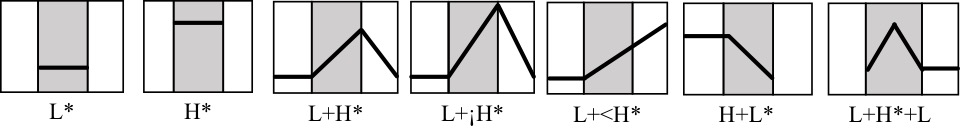
\includegraphics[width=\textwidth]{figures/pes-img1.png}
   \caption{\label{fig:pes:1}Inventory of pitch accents in Porte{\~n}o Spanish (according to \citealt{Gabriel2010incollection}).}
\end{figure}
  
The corpus subset containing PS was analyzed and all instances of pitch accents were duly noted. Next, each instance was examined to see if the subject was separated from the rest of the material by a \isi{boundary tone}. \citet{Gabriel2010incollection} assume three monotonal (L, H, downstepped-high !H) boundary tones and one bitonal (HL) \isi{boundary tone}. All of them are attested at the end of intonational phrases (IPs) as well as at the end of intermediate phrases (ips) (\figref{fig:pes:2}).\footnote{Additionally, \citet{Gabriel2011} observe three boundary realizations H\textminus{}, HL\textminus{}, and LH\textminus{} at the intermediate phrasal boundaries (break index 3) after subject (besides some other boundary cues such as pitch reset and pre-boundary upstep). These \isi{phonetic} differences were not relevant for the present study.
}


\begin{figure}[t]
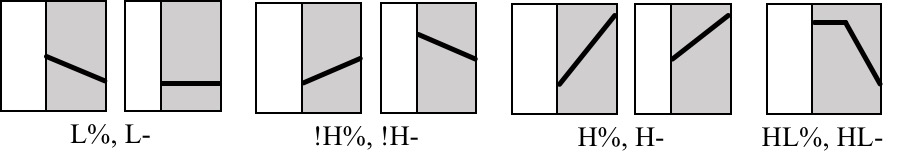
\includegraphics[width=.8\textwidth]{figures/pes-img2.png} 
  \caption{Inventory of boundary tones in Porte{\~n}o Spanish (according to \citealt{Gabriel2010incollection}).}
  \label{fig:pes:2}
  \end{figure}
  
As can be surmised, \textit{Porte{\~n}o} pitch accents as well as boundary tones have different distributional properties. For instance, the \isi{tritonal pitch accent} L+H*+L is commonly found in the nuclear position, where it expresses emphasis or marks a focus (see \citealt{Gabriel2010incollection,Feldhausen2011}). The realization of L+H* (formerly called ``early peak'') is typical of \isi{prenuclear} accents in this variety, whereas the L+<H* (formerly called ``late peak'') is found sporadically in the \textit{Porte{\~n}o} data (see \citealt{Peskova2012}). Since pronominal subjects occur mainly in the \isi{prenuclear} (sentence-initial) position (92\% of the PS in the data of the present study),\textsuperscript{} their \isi{tonal realization} is expected to have an L+H* (with the peak located at the end of the accented \isi{syllable}) or occasionally L+<H* (with the peak aligned with the postaccentual \isi{syllable}).\footnote{The \isi{pitch accent} L+H*—associated with the PS in sentence-initial or preverbal position—was also found in the nuclear position when it was followed by an intermediate \isi{boundary tone} (e.g. \textit{Yo} \textsuperscript{[L+H* H\textminus{}]} \textit{nunca hacía los deberes}, \figref{fig:pes:3}).}  Another possible \isi{prenuclear accent} is a H*, found in different sentence types especially at the very beginning of utterances. Additionally, there are certain ``intermediate'' cases, where, for instance, the \isi{pitch movement} is falling in the posttonic \isi{syllable} but the peak is located in the onset of the nucleus of the same \isi{syllable}. Is this still an L+H* or is it an L+<H*? According to the definition given by the \ili{Spanish} ToBI system, it should be L+<H* (as the peak is located outside the accented \isi{syllable}), yet the realization is perceived very differently from a typical L+<H* as described by Sp\_ToBI. The rising \isi{pitch movement} can also be either very brusque or very moderate. Nevertheless, all such pitch realizations were labeled L+H* in the present study. As a rich variation in pitch accents was attested in the data, the present study applied the \ili{Spanish} ToBI labels using broad \isi{phonetic transcription} (see \citealt{Hualde2016}) and in accordance with the following criteria. If a \isi{pitch accent} associated with the PS was rising, it was labeled L+H* or L+<H* (depending on the \isi{pitch movement} in the posttonic \isi{syllable}). If the \isi{pitch accent} had a high or a low plateau, it was labeled H* or L*, respectively. If the \isi{pitch accent} was falling within the accented \isi{syllable}, it was labeled H+L*. And finally, if the \isi{pitch accent} had a \isi{rising-falling pitch} contour within the stressed \isi{syllable}, the label L+H*+L was used.\footnote{A reviewer has rightfully objected to the fact that \isi{prosodic} annotation was carried out by only one person (the author) and therefore a subjective element may well have been present in the labeling. While this is true, the author is an experienced labeler of Argentinean \isi{intonation}, and in this instance whenever ambiguous data were encountered they were discussed with other trained ToBI labelers (who were also experts in the Argentinean variety). Moreover, the results from previous research showed generally a high agreement between the trained labelers and give evidence to regard the ToBI systems as a standard reference for \isi{prosodic} annotation (see \citealt{Escudero2012} for \ili{Catalan} ToBI; \citealt{Feldhausen2016} for \ili{Spanish} ToBI). However, I do not rule out the possibility that such tests will be carried out on this data prior to any future research, not only for the ToBI labeling, but also for the IS categories proposed here.}

The advantage of ToBI labels is that in principle they provide simplified representations of tonal events and are easy to read. However, several difficulties were encountered in applying the ToBI labels to \isi{spontaneous speech}. By way of contrast, we first show in Figures \ref{fig:pes:3} and \ref{fig:pes:4} examples of the F0 contour for a \isi{rising pitch accent} (L+H*) associated with the monosyllabic PS \textit{yo} (‘I’) that conforms to the archetypical pattern: the rise starts at the onset of the \isi{syllable} and ends at the end of that \isi{syllable}; the difference between the minimal and maximal pitch is 80 Hz (6 ST) (\figref{fig:pes:3}), and 100 Hz (7.5 ST) (\figref{fig:pes:4}).

  
\begin{figure}[p]
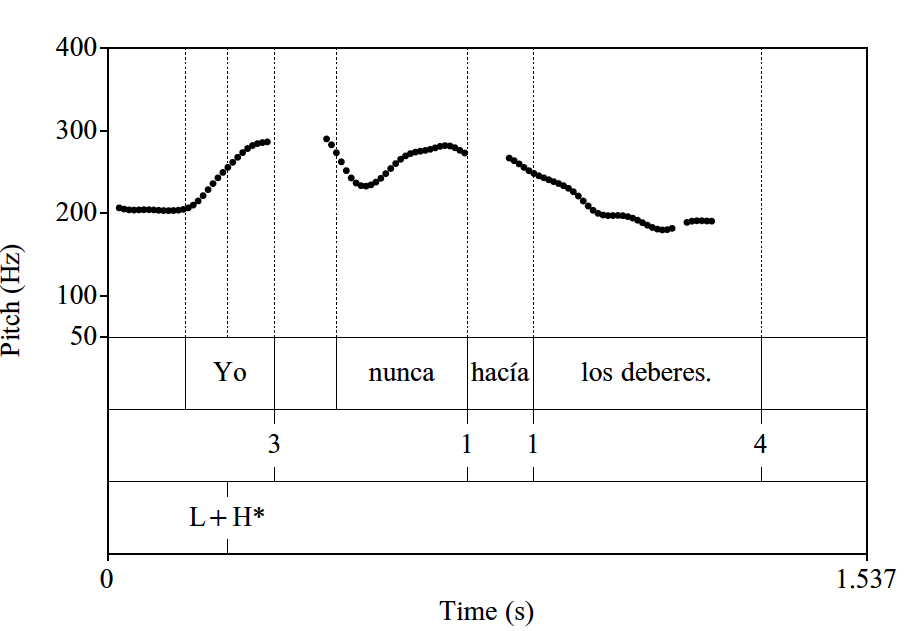
\includegraphics[width=.8\textwidth]{figures/pes-img3.png}
\caption{F0 contour of the utterance \textit{\textbf{Yo} nunca hacía los deberes} (‘I never did my homework’), with a rising pitch accent on the pronoun \textit{yo}.\label{fig:pes:3}} 
  \end{figure}
  
\begin{figure}[p]
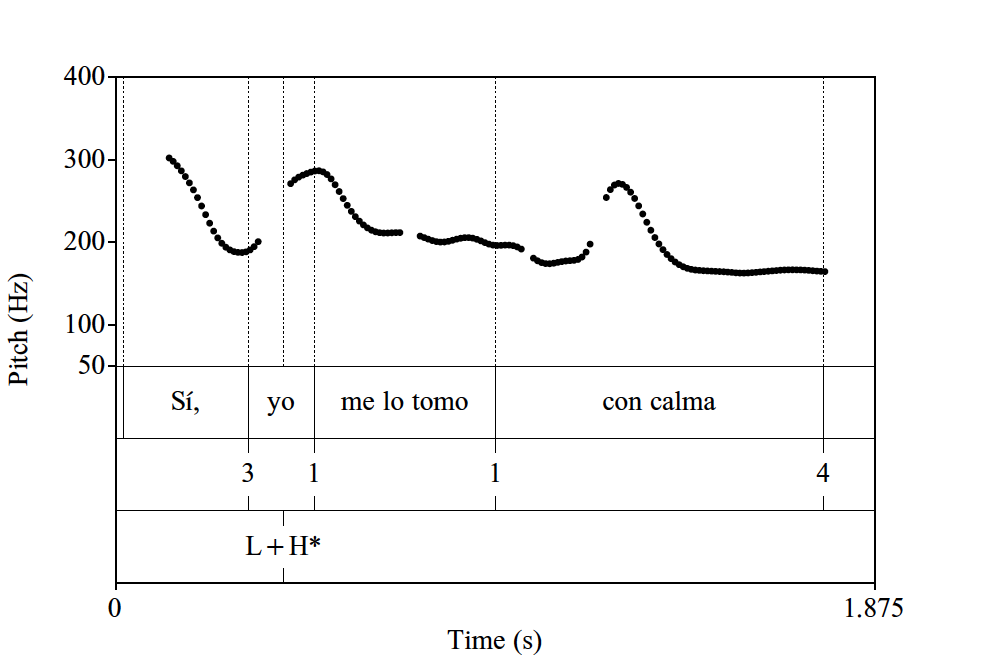
\includegraphics[width=.9\textwidth]{figures/pes-img4.png}
\caption{F0 contour of the utterance \textit{\textbf{Yo} me lo tomo con calma} (‘I take it easy’), with a rising pitch accent on the pronoun \textit{yo}.\label{fig:pes:4}} 
\end{figure}
  
On the other hand, \isi{prosodic} annotation proved more difficult for utterances from the corpus like \textit{yo tomo mucho mate}, illustrated in \figref{fig:pes:5}. Here the pitch reaches a high plateau (H) (166–162 Hz), but no preceding initial dip is observed or perceived clearly either, since the \isi{voiceless} palato-alveolar fricative [ʃ] in the word \textit{yo} ([ʃo]) causes gaps in the acoustic report and has no definite pitch.

  

\begin{figure}[p]
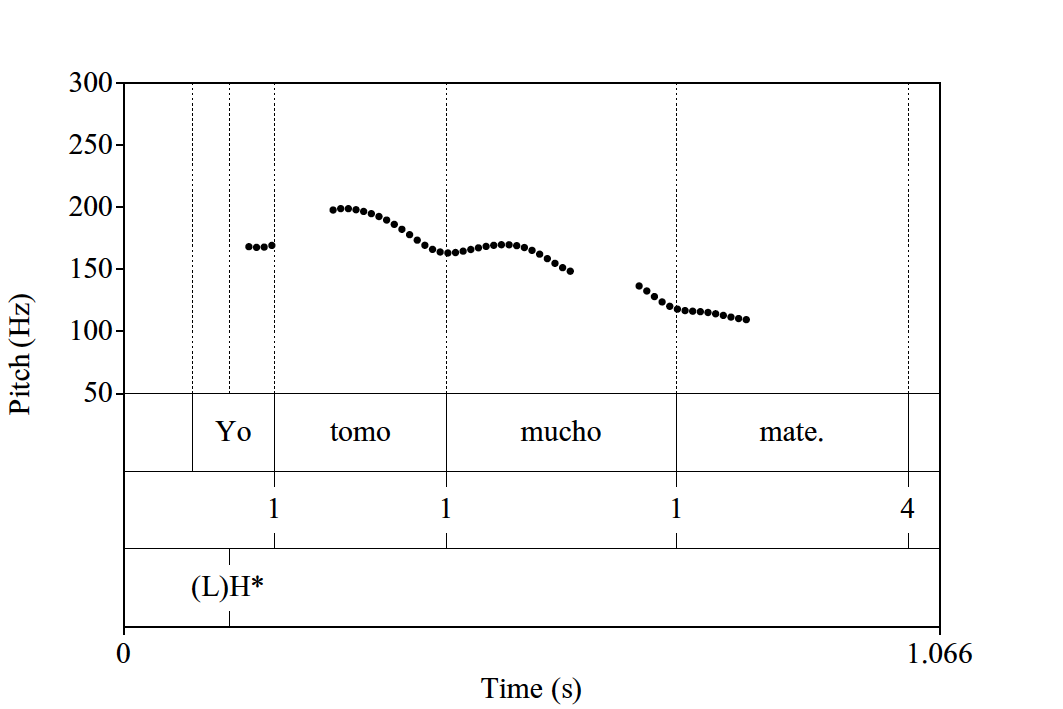
\includegraphics[width=\textwidth]{figures/pes-img5.png}
\caption{F0 contour of the utterance \textit{\textbf{Yo} tomo mucho mate} (‘I drink a lot of mate’), with a high pitch accent on the pronoun \textit{yo}.\label{fig:pes:5}}
  \end{figure}
  
  \begin{figure}[p]
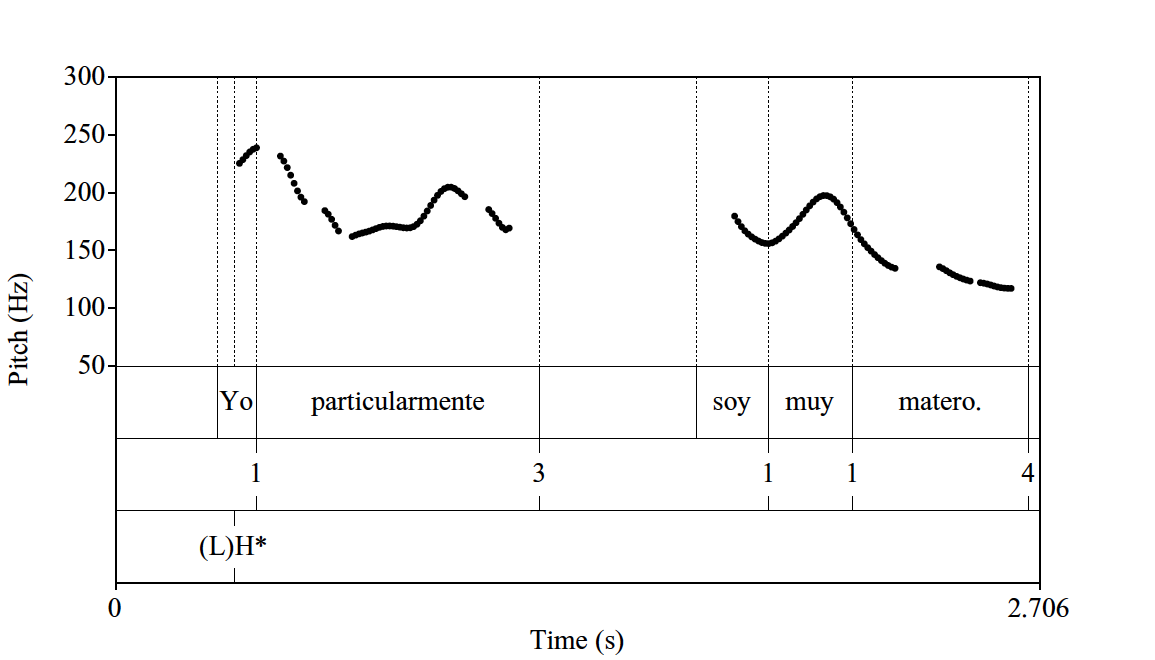
\includegraphics[width=\textwidth]{figures/pes-img6.png}
\caption{F0 contour of the utterance \textit{\textbf{Yo} particularmente soy muy matero} (‘I am particularly fond of {mate}’), with a very slightly rising pitch accent on the pronoun \textit{yo}.\label{fig:pes:6}}
\end{figure}
  
Besides \isi{voiceless} segments, monosyllabic pronouns such as \textit{yo} (‘I’), \textit{él} (‘he’), or \textit{vos} (‘you’) followed by another stressed \isi{syllable} (such as [ˈʃo.ˈto.mo]) represented another difficulty in the analysis of the spontaneous data. Such (tonal) clash contexts can trigger a timing reorganization and earlier peak placement of the accents involved, or reduction of the two underlying gestures, resulting in a single one \citep{Prieto1995}. This means that in such contexts the speaker does not implement both pitch accents phonetically or that the low target from the default L+H* is not realized overtly because it lacks \isi{phonetic} material.





\figref{fig:pes:6} shows another example of the pronoun \textit{yo} produced by the same speaker. In comparison to the previous example, we observe here that the first \isi{pitch accent} on the monosyllabic pronoun \textit{yo} displays a high \isi{pitch movement} that is slightly rising (222–241 Hz; 1.4 ST). Again, there is no \isi{pitch movement} in the \isi{voiceless} consonant, but the short rising movement is clearly perceived. In music, for example, such a difference corresponds approximately to a difference between the notes A and B in the third octave. Is it a rising (L+H*) or just a high target (H*)? All the intermediate cases found in the data were somewhat tricky, but very similar to the variation one sees, for instance, in vowels, which can be observed by measuring their formants (frequency components). Vowels very often display a large dispersion and variability (which depend on the context, speech rate, etc.), and they may even overlap each other, making it impossible to draw clear boundaries between them. Considering all the difficulties, the present paper will argue that though the tonal event (\figref{fig:pes:5}; \figref{fig:pes:6}) is a H* from the \isi{phonetic} perspective, it is an L+H* from the phonological perspective.

\section{Results}
\label{sec:pes:4}
This section presents results of the analysis of tonal realizations of the expressed subject with different discourse-pragmatic functions (\textit{N=}976). It should be emphasized that the IS functions of overt PS were defined according to the pre-established categories, after the intonational properties of the overt PS were described. This step was necessary especially for identifying ``emphatic'' (here: focal) subjects. We will see that there are clear intonational differences between focus and topic: whereas preverbal focal PS as well as one third of the right-shifted focal PS in the present data set had a F0 \isi{rising-falling contour} with its peak located within the accented \isi{syllable}, the prevailing \isi{tonal realization} of all types of topics was a \isi{rising tone}. However, we also observed a high degree of variation regarding the type of pitch accents associated with topics.\pagebreak

The distribution of all overt PS in the corpus was as follows: Aboutness-shift topic (45\%) > Familiar topic (31\%) > \is{topic!contrastive}contrastive topic (11\%), Focus (8\%) > Disambiguating topic (5\%). These percentages clearly show that instances of the obligatory expression of PS (F, Tc, Td) were much less common than instances of the variable (i.e. omissible) PS (Ta, Tf).
  
\subsection{Pronominal subjects as focus}
\label{sec:pes:4.1}
Seventy-six subject pronouns expressing focus appeared in postverbal (clause-final) (\textit{N}=43) or preverbal position (\textit{N=}33) (\figref{fig:pes:7}).\footnote{Seven cases of preverbal focus and four cases of postverbal focus were excluded from the analysis.} In both of these positions, the PS bear the \isi{nuclear accent}. As all focal PS must be overtly realized in \ili{Spanish}, different types of focus were not distinguished. However, the PS as a \is{focus!contrastive}contrastive focus prevailed; in both preverbal and postverbal position.


\begin{figure}
% %  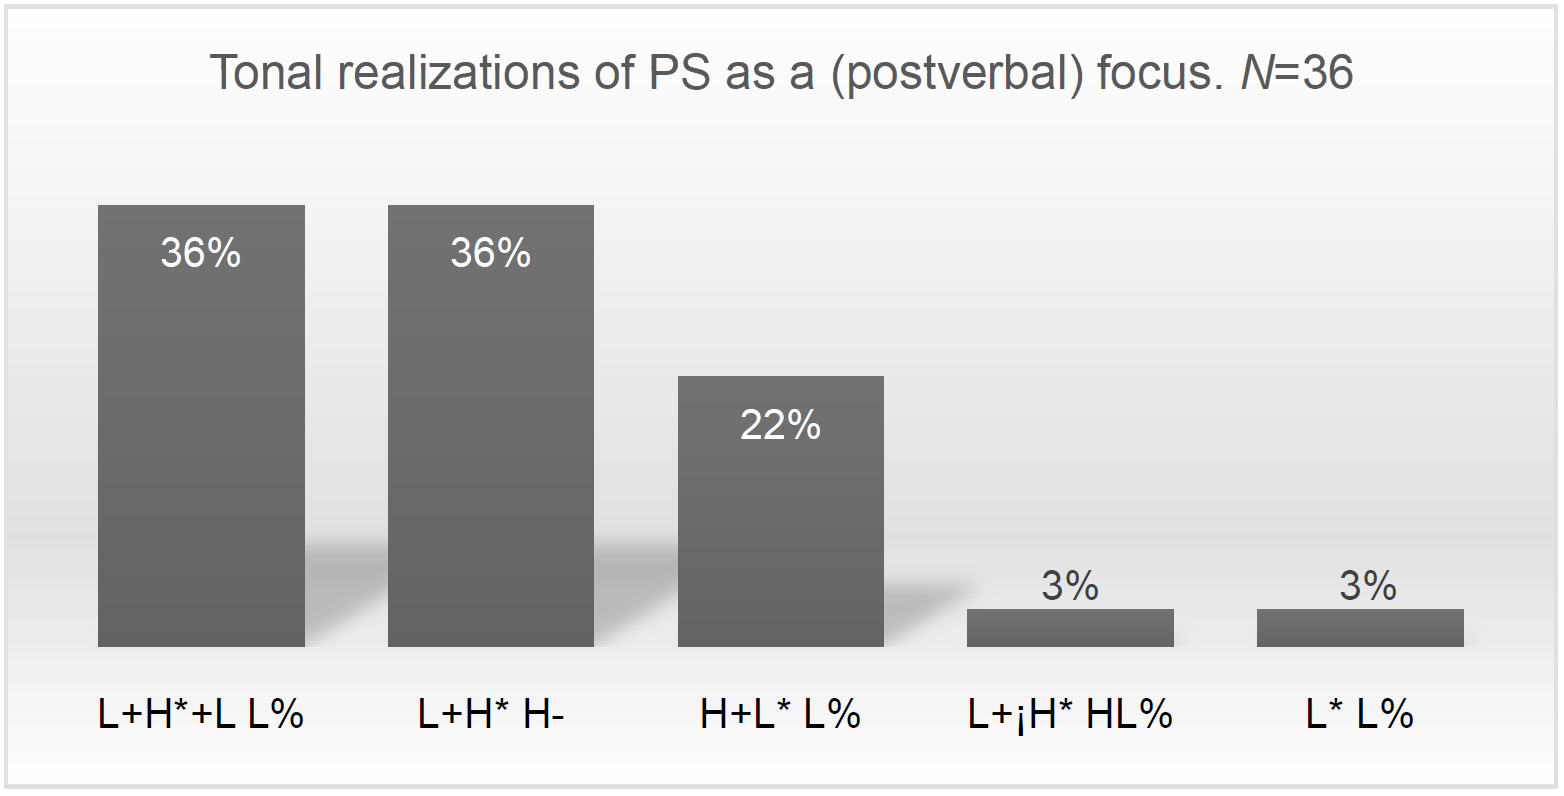
\includegraphics[width=\textwidth]{figures/pes-img7.png} 
\barplot{}{\%}{L+H*+L~L\%,L+H*~H\textminus{},H+L*~L\%,L+¡H*~HL\%,L*~L\%}{
  (L+H*+L~L\%,36)
  (L+H*~H\textminus{},36)
  (H+L*~L\%,22)
  (L+¡H*~HL\%,3)
  (L*~L\%,3)
}
\caption{Percentages for different pitch accents of PS as focus (in postverbal position).\label{fig:pes:7}}
\end{figure}

\figref{fig:pes:8} offers an example of the pronoun subject \textit{nosotras} (‘we-F’) in postverbal and clause-final position.\footnote{The context of this example was as follows:

\begin{exe}
\exi{(i)}
\textit{No terminábamos de entender cuál era la línea, no solamente del colegio, sino la que teníamos que seguir \textbf{nosotras}}.\\
(‘We could not understand what the line was, not only in the school, but also the one WE had to follow.’)
\end{exe}\vspace*{-\baselineskip}} 
The pronoun shows a typical \isi{tritonal pitch accent}, which displays an arc pattern within the metrically strong \isi{syllable} -\textit{so}- and is characterized by and perceived as a rising-falling tonal movement.


\begin{figure}[p]
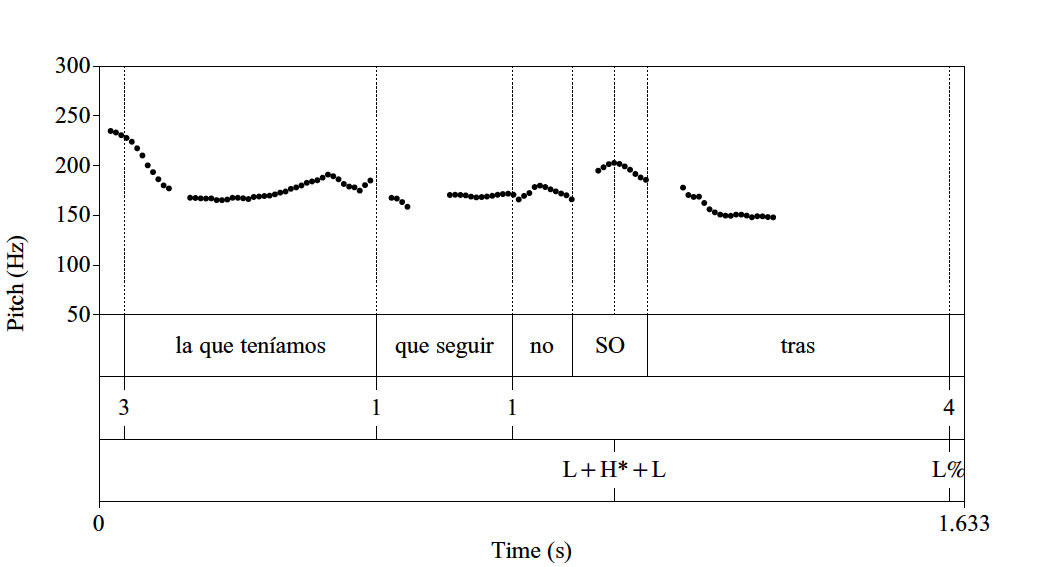
\includegraphics[width=\textwidth]{figures/pes-img8.png}
\caption{F0 contour of the utterance \textit{la que teníamos que seguir \textbf{nosotras}} (‘the one we had to follow’) with a postverbal subject as focus (break index 4), realized with an L+H*+L (L\%).\label{fig:pes:8}}
\end{figure}

\begin{figure}[p]
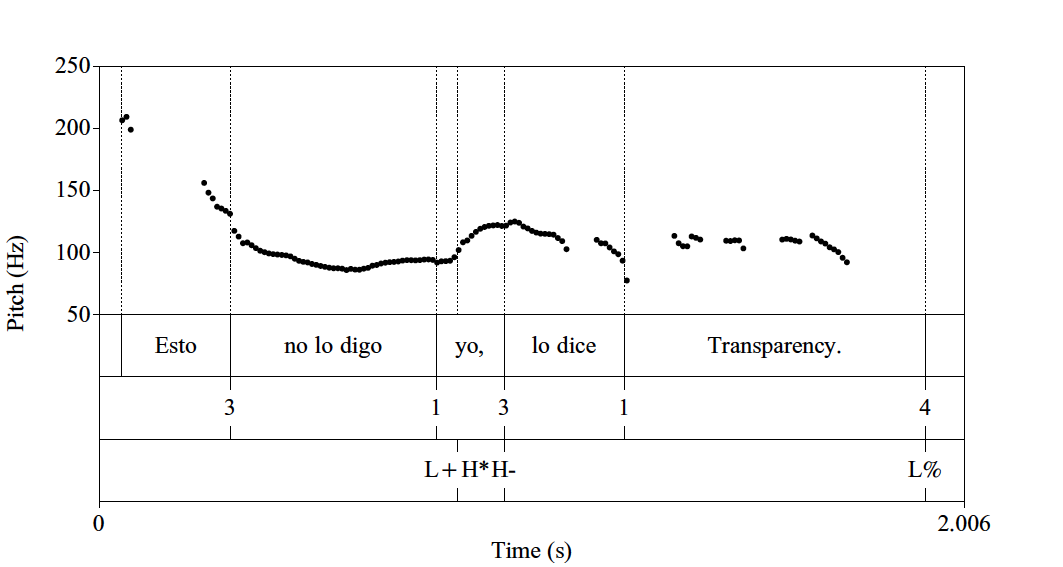
\includegraphics[width=\textwidth]{figures/pes-img9.png}
\caption{F0 contour of the utterance \textit{Esto no lo digo \textbf{yo}, lo dice Transparency} (‘It’s not me who says this, it’s Transparency’) with a postverbal subject as focus (BI 3), realized with an L+H* (H\textminus{}).\label{fig:pes:9}}
\end{figure}%%\clearpage

Focal subjects in the data were realized as a \is{tritonal pitch accent}tritonal (L+H*+L), a falling (H+L*), or a low (L*) \isi{pitch contour} if they appeared at break index 4 (L\%). If the subject appeared at the end of an intermediate phrase (H\textminus{}), it was realized as an L+H* (\figref{fig:pes:9}).

As for the tonal configuration L+¡H* HL\%, this pattern appeared in only one instance in the data set, the interrogative sentence \textit{¿Te dijo} \textbf{\textit{ella}}? (in the context \textit{Who told you that?} ‘\textit{Did SHE} \textit{tell you that?}’). The \isi{boundary tone} HL\% is typical for yes-no questions in the variety under study (see \citealt{Gabriel2010incollection}).

Since \ili{Spanish} exhibits a greater flexibility in word order and the focus is usually shifted to the rightmost position of the sentence, it shows less ``flexibility in the placement of the \isi{nuclear accent} (or main phrasal stress)'' (\citealt[358]{Hualde2015}). Nevertheless, the PS is realized with an L+H*+L (\figref{fig:pes:10}) in cases of preverbal focus subject placement.\footnote{The context of this example is as follows:

\begin{exe}
\exi{(ii)}\textit{Yo sí vivo en Buenos Aires y actúo en Buenos Aires y juego en Buenos Aires, no puedo hablar como entrerriano no por no estar orgulloso de mi pueblo sino para entrar en sintonía con la gente con la que \textbf{yo} estoy trabajando.}\\
(‘If I live and act in Buenos Aires and play in Buenos Aires, I cannot speak as a person from Entre Ríos, not because I’m not proud of my home town but rather so that I can get along with the people I am working with.’)
\end{exe}

At first glance, the second pronoun \textit{yo} is omissible. However, the speaker wants to highlight the subject and this is made clear in the \isi{intonation}, since the \isi{pitch movement} shows a \is{tritonal pitch accent}tritonal pattern on \textit{yo} and subsequent postfocal deaccentuation (on \textit{estoy trabajando}). For this reason, the pronoun \textit{yo} is assumed to be a focus.} Only five such instances of focal preverbal subjects were found in the data. 


\begin{figure}
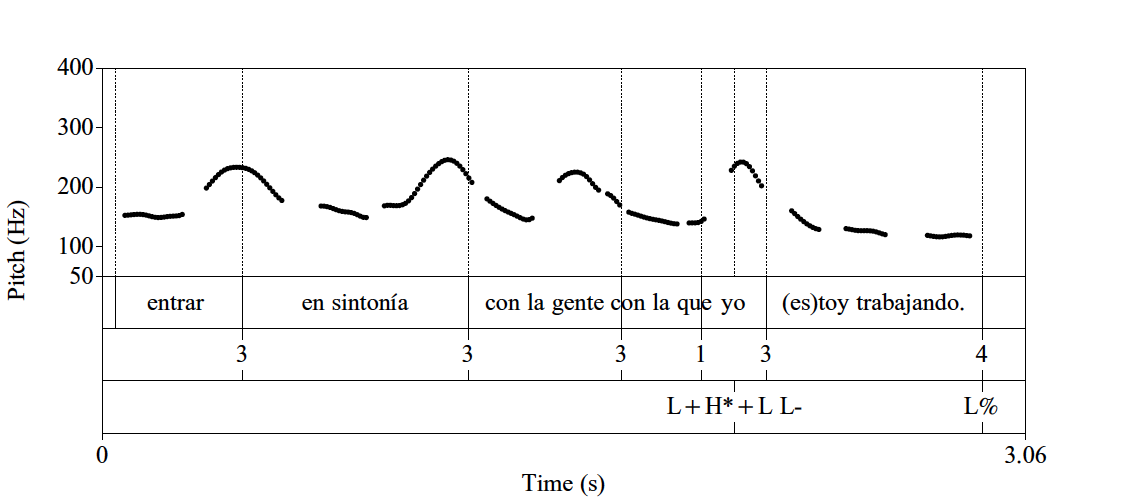
\includegraphics[width=\textwidth]{figures/pes-img10.png}
\caption{F0 contour of the utterance \textit{para entrar en sintonía con la gente con la que \textbf{yo} estoy trabajando} (‘to get along with the people who I am working with’) with a preverbal PS as focus, realized with an L+H*+L (L\textminus{}).} 
\label{fig:pes:10}
\end{figure}

Besides \isi{prosodic} or syntactic marking of focus in \ili{Spanish}, other strategies may be used to express focus, namely cleft constructions (e.g. \textbf{\textit{Yo}} \textit{soy quien te llamó}, ‘It was me who called you’) or focusing adverbs associated with the PS such as \textit{también} (‘also’)  or \textit{por lo menos} (‘at least’). In these cases, the subject is realized predominantly with a rising L+H* tone, which can but does not have to be separated by a \isi{high boundary} tone from the rest of the material (H\textminus{}) (\figref{fig:pes:11}; \figref{fig:pes:12}). 

\begin{figure}
\caption{Percentages for different pitch accents of PS as a focus (in preverbal position).}
\barplot{}{\%}{L+(¡)H*+L~L\textminus{},L+H* (H\textminus{}),L*,H*}{
  ({L+(¡)H*+L~L\textminus{}},0)
  ({L+H* (H\textminus{})},67)
  (L*,21)
  (H*,12)
}
\label{fig:pes:11}
\end{figure}

  
\begin{figure}
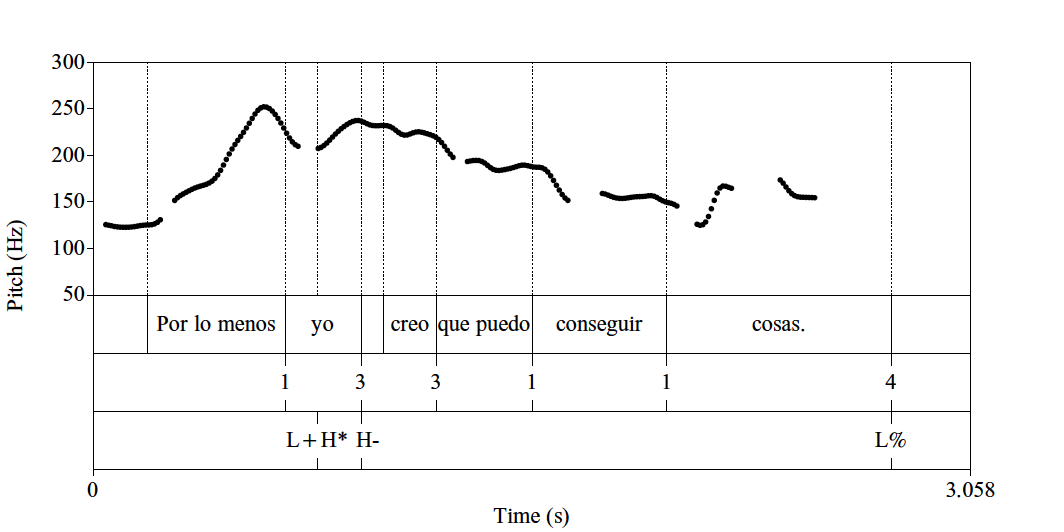
\includegraphics[width=\textwidth]{figures/pes-img12.png}
\caption{F0 contour of the utterance \textit{Por lo menos \textbf{yo} creo que puedo conseguir cosas} (‘At least I believe that I can achieve things’) with a focusing adverb and a preverbal PS realized with an L+H* (H\textminus{}).\label{fig:pes:12}}
\end{figure}

\subsection{Pronominal subjects as Topics} 
\label{sec:pes:4.2}
Most overtly realized PS in the data were topics, with the following distribution: Ta (\textit{N}=442), Tf (\textit{N}=304), Tc (\textit{N}=110), Td (\textit{N}=44) (see \figref{fig:pes:13}).\footnote{Sixty-one PS expressing a topic were excluded from analysis due to poor sound quality.}\largerpage[-1]

\begin{figure}
% 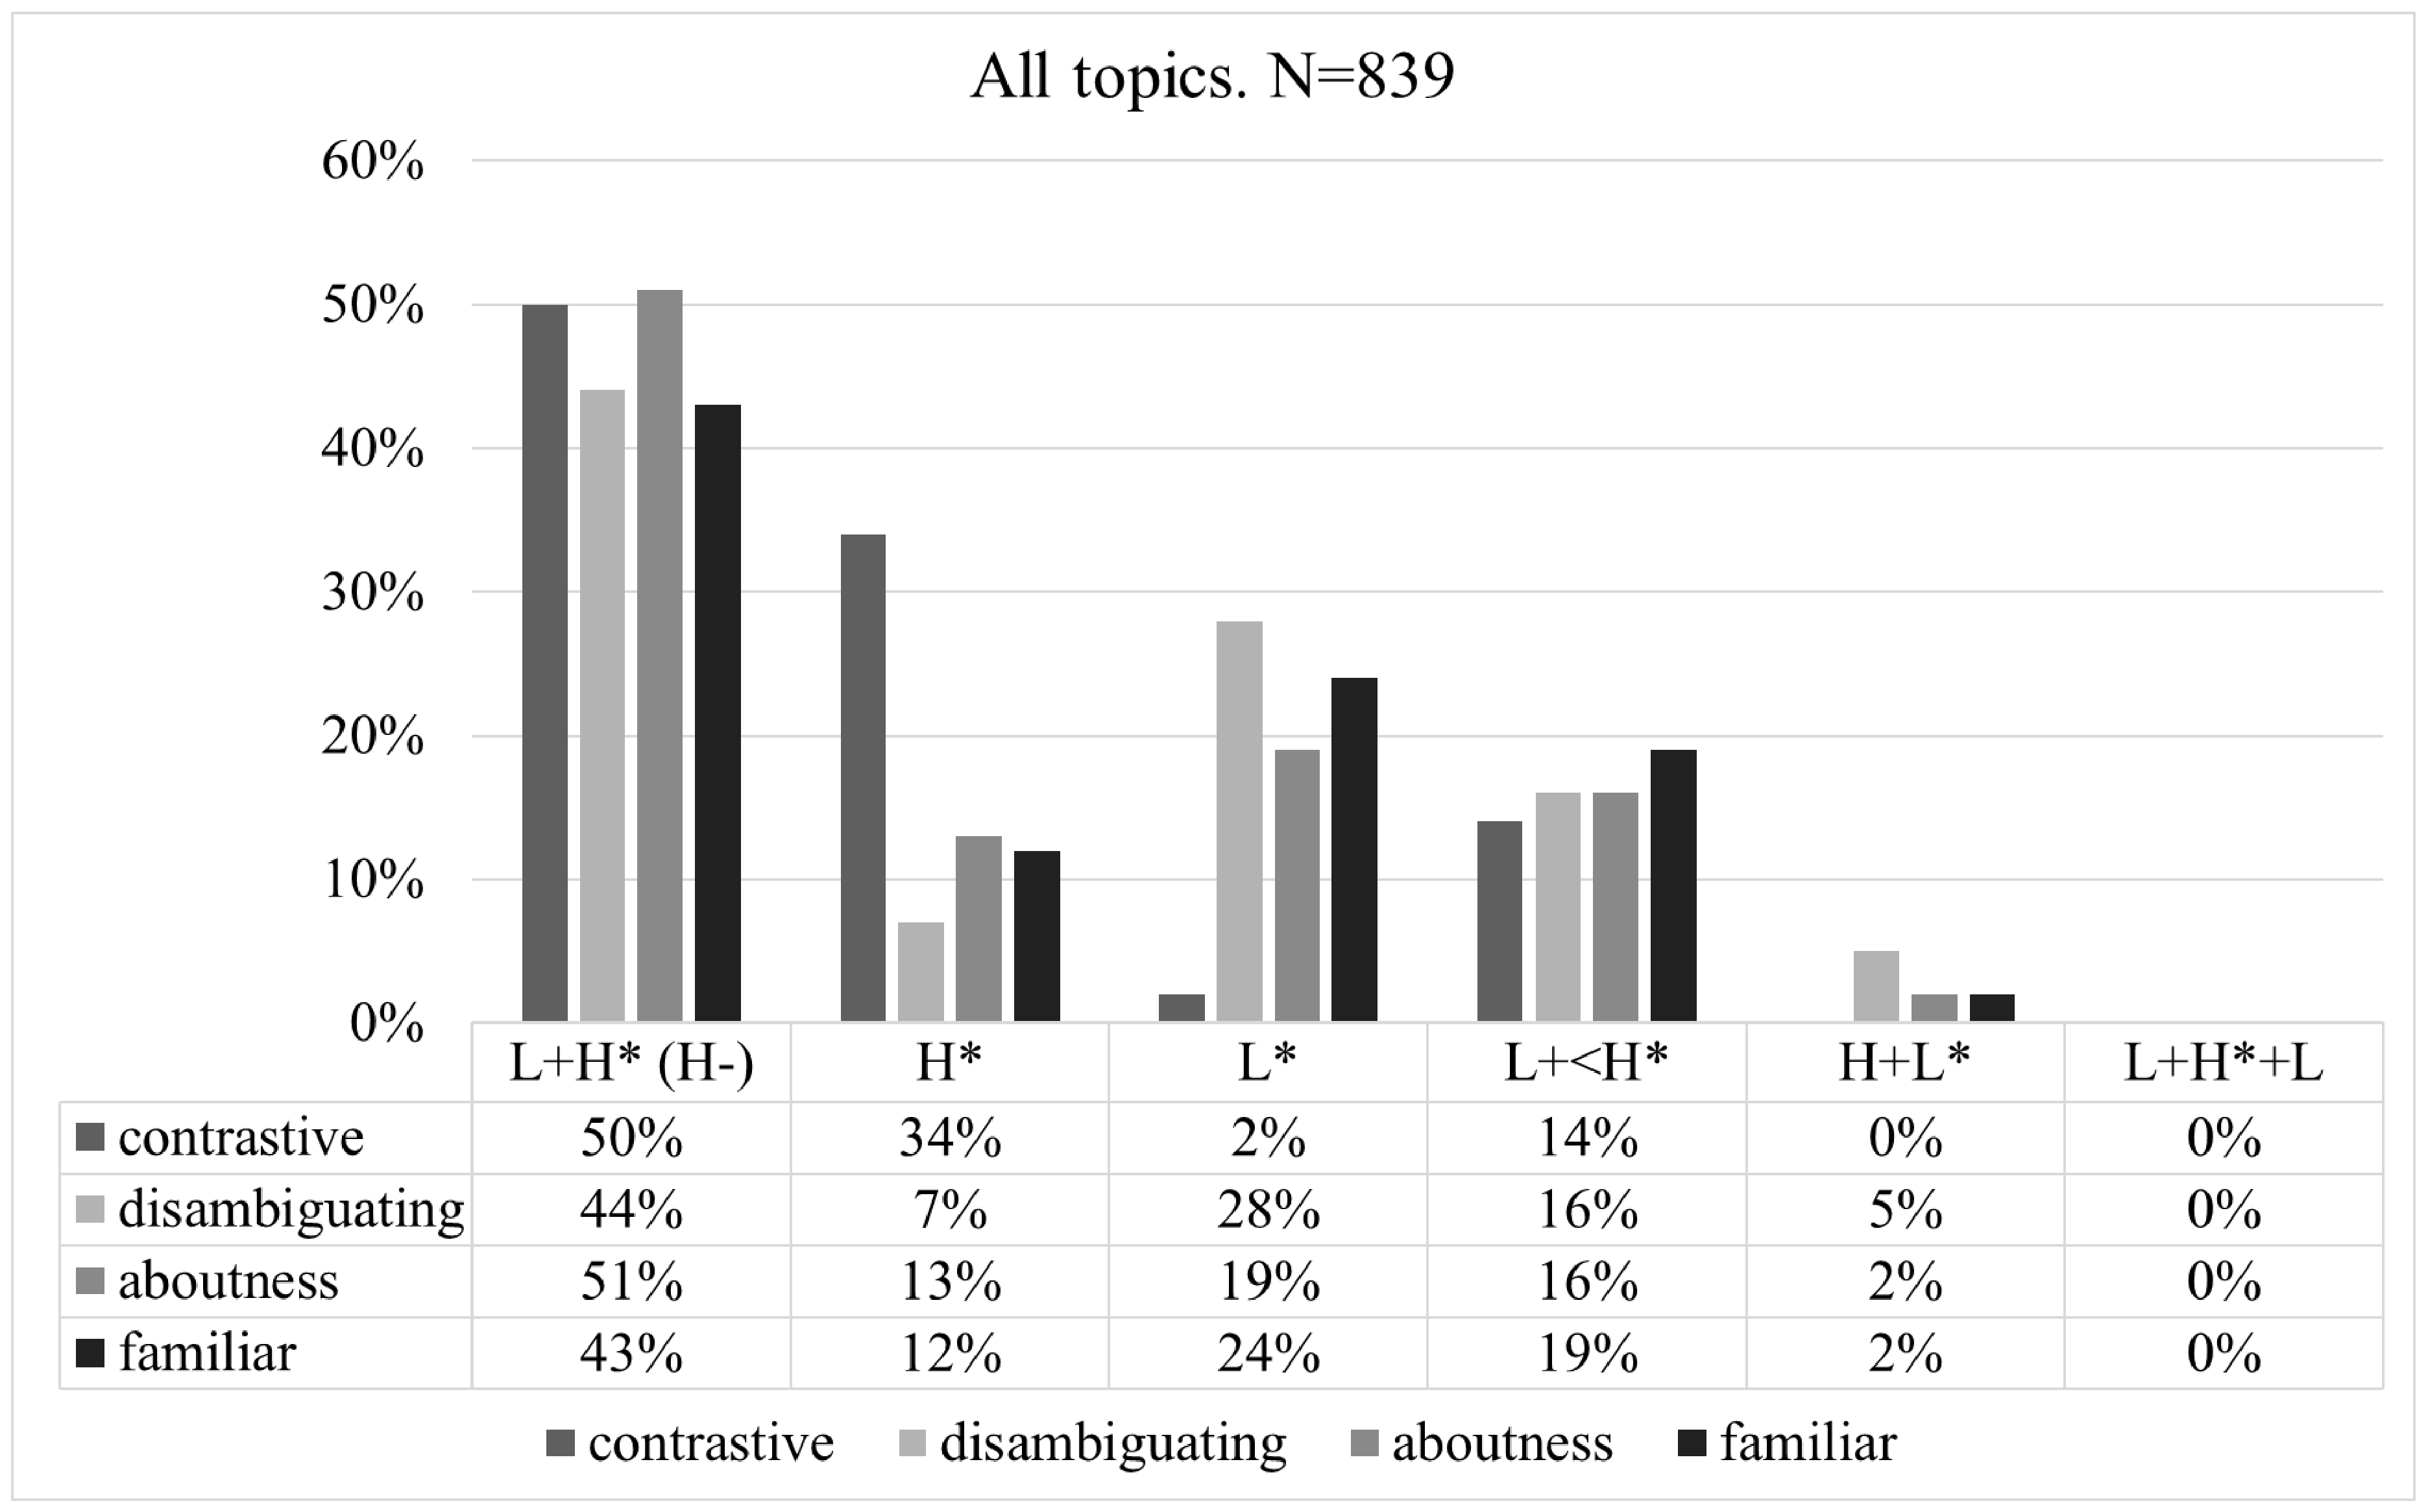
\includegraphics[width=\textwidth]{figures/pes-img13.eps}
\caption{Tonal realizations of different types of topics.\label{fig:pes:13}} 
  \begin{tikzpicture}
    \begin{axis}[
	xlabel={},  
	ylabel={\%}, 
	axis lines*=left, 
        width  = \textwidth,
	height = .3\textheight,
    	nodes near coords, 
	xtick=data,
	x tick label style={},
	xtick distance={1000},
	enlarge x limits=true,
	ymin=0,
	xticklabels={L+H*~(H−),H*,L*,L+\textless H*,H+L*,L+H*+L},
	ybar,
	legend cell align=left,
	area legend
	]
	\addplot+[black,pattern=dots,pattern color=black,draw=black] coordinates {(0,50) (1,34) (2,2) (3,14) (4,0) (5,0)};
	\addplot+[black,pattern=horizontal lines,pattern color=black,draw=black] coordinates {(0,44) (1,7)  (2,28) (3,16) (4,5) (5,0)};
	\addplot+[black,pattern=north east lines,pattern color=black,draw=black] coordinates {(0,51) (1,13)  (2,19) (3,16) (4,2) (5,0)};
	\addplot+[black,pattern=crosshatch,pattern color=black,draw=black] coordinates {(0,43) (1,12)  (2,24) (3,19) (4,2) (5,0)};
	\legend{contrastive,disambiguating,aboutness,familiar}
    \end{axis} 
  \end{tikzpicture} 
% \todo[inline]{redraw based on values - THIS IS A NEW VERSION. OK?}
\end{figure}

All the types of topics clearly preferred the \isi{rising tone} L+H*, which could occur optionally with a \isi{high boundary} tone (H\textminus{}) (\figref{fig:pes:14}).\footnote{In this example, the speaker was answering the simple question \textit{¿Qué hacés?} (‘What do you do?’). Notice that the pronoun \textit{yo} is very long and sharply rising; its function seems to correspond to an introductory discourse marker along the lines of ``as for me''.} There were no significant differences between the topic types in terms of this \isi{pitch accent} (χ\textsuperscript{2}(3)=4.324, p=0.229). The findings that \ili{Spanish} can also sometimes \isi{accent} (i.e. realize a \isi{rising pitch accent} on) old information (e.g. familiar topics) and that the words can lack a \isi{pitch accent} in a \isi{prenuclear position} are consistent with some previous studies (see, e.g., \citealt{Cruttenden1993,Face2003}).

  We should specify that the \isi{boundary tone} or pause after a subject-topic is not obligatory and thus does not represent any cue for distinguishing among different kinds of topics. It was attested in only 29\% of the instances found in the present data set. However, the monosyllabic pronouns (\textit{yo}, \textit{vos}, \textit{él}; ‘I, you (informal), he’) exhibited fewer boundary tones (14\%) in comparison to ``longer'' pronouns (\textit{nosotros}, \textit{ustedes}, \textit{ella}, \textit{ellos}; ‘we, you (formal), she, they’) (49\%).\footnote{\citet{Feldhausen2010bantu} found that, similarly to pronominal subjects, left-dislocated objects are also not always marked with a \isi{boundary tone} in \textit{Porte{\~n}o} \ili{Spanish}. Other varieties of \ili{Spanish}, however, may show a different picture. For example, \citet{Feldhausen2016} shows that left dislocations (objects) in Peninsular \ili{Spanish} require an obligatory boundary, independently of the length of the dislocated element. For \isi{prosodic} marking in different \ili{Romance} varieties see \citet{DImperio2005}; \citet{Frota2007}; and \citet{Feldhausen2010nequen}.}

Another example of a topic with a typically \isi{rising pitch accent}, associated with the metrically strong \isi{syllable} of the PS, is illustrated in \figref{fig:pes:15}.\largerpage[2]

  
\begin{figure}[H]
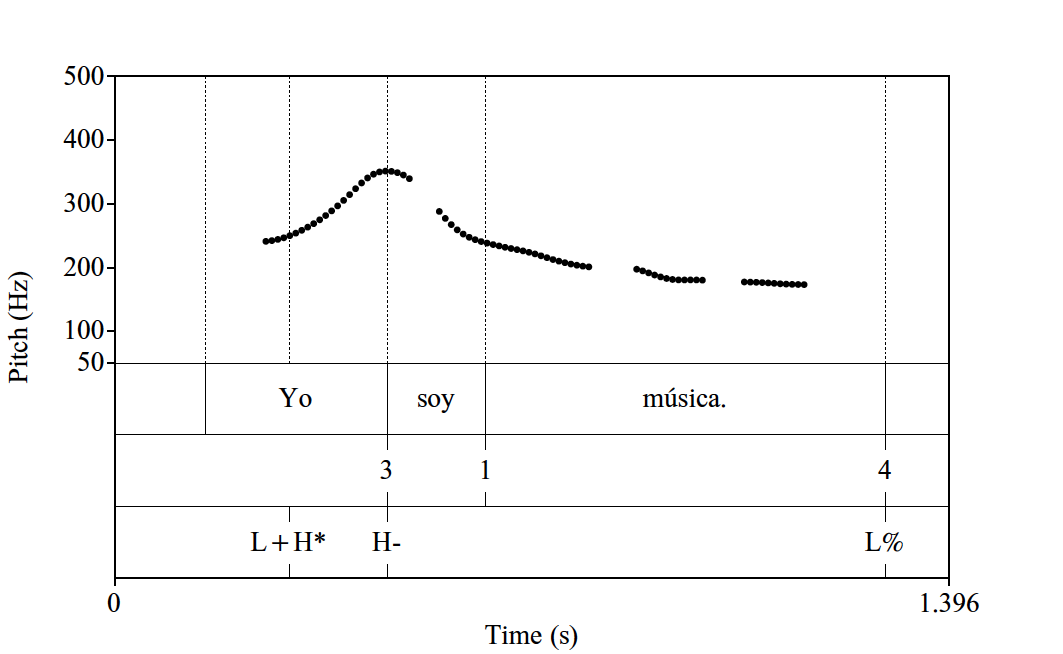
\includegraphics[width=.9\textwidth]{figures/pes-img14.png}
\caption{F0 contour of the utterance \textit{\textbf{Yo} soy música} (‘I am a musician’) with a preverbal PS as a familiar topic, realized with an L+H* (H\textminus{}).\label{fig:pes:14}}
\end{figure}\clearpage

\begin{figure}[p]
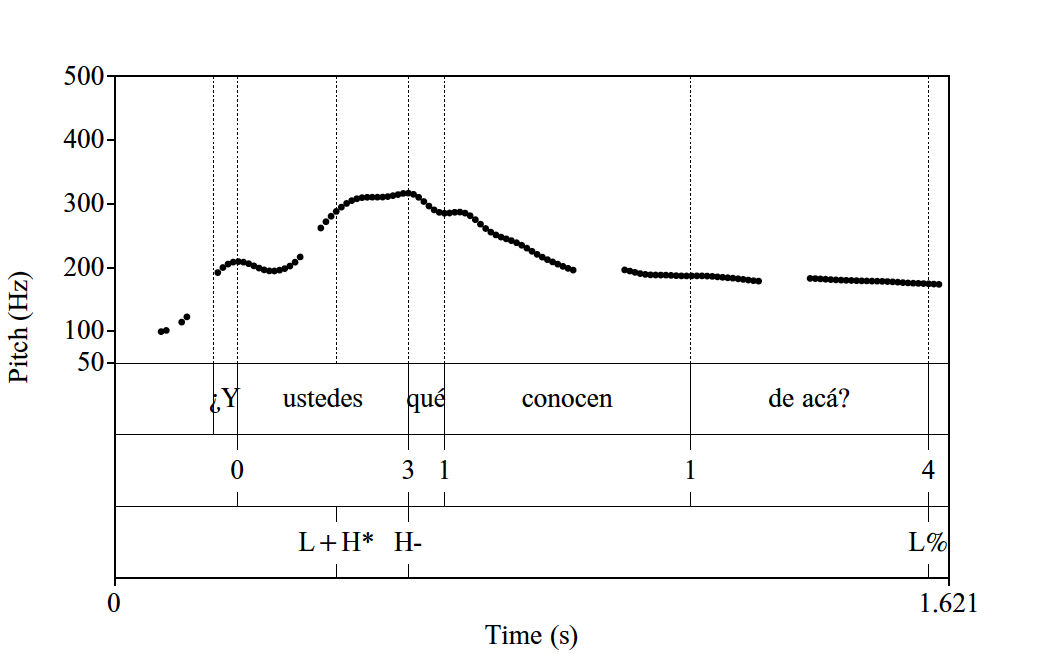
\includegraphics[width=\textwidth]{figures/pes-img15.png}
\caption{F0 contour of the utterance \textit{¿Y \textbf{ustedes} qué conocen de acá?} (‘And you, what do you know here?’) with a preverbal PS as an aboutness-shift topic, realized with an L+H* (H\textminus{}).\label{fig:pes:15}}
\end{figure}

\begin{figure}[p]
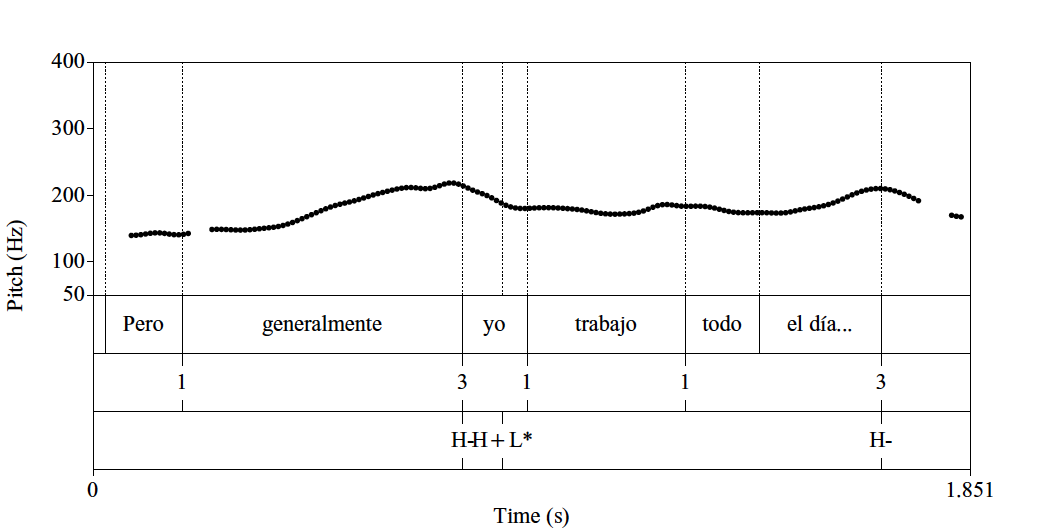
\includegraphics[width=\textwidth]{figures/pes-img16.png}
\caption{F0 contour of the utterance \textit{Pero generalmente \textbf{yo} trabajo todo el día} (‘But in general, I work all day long’) with a preverbal PS as a familiar topic, realized with a H+L*.\label{fig:pes:16}}
\end{figure}

Further tonal realizations of PS as a topic were a \isi{high tone} (H*), a \isi{low tone} (L*), or a \isi{rising tone} with a displaced peak (L+<H*). The falling tone (H+L*) was atypical and occurred only after a \isi{high boundary} tone (\figref{fig:pes:16}).\footnote{In this example, as in other similar cases, we observe no pitch excursion (due to the falling interpolation). The label H+L* serves here a purely practical purpose, i.e., it helps to distinguish and systematize the contours encountered in the data.}\largerpage[2]

  



Moreover, one difference between \is{topic!contrastive}contrastive topics and other types of topics was observed. Whereas the second predominant \isi{pitch accent} of \is{topic!contrastive}contrastive topics was a \isi{high tone} (\figref{fig:pes:17}),\footnote{The context of this example is as follows:
\begin{exe}
\exi{(iii)} \textit{Sí, aparte a los extranjeros no les gusta amargo. A mí, \textbf{yo} lo tomo amargo.}\\
(‘Generally, foreigners do not like it {[}\textit{mate}{]} bitter. As for me, \textit{\uline{I}} drink it bitter.)’
\end{exe}\vspace*{-\baselineskip}} disambiguating, aboutness, and familiar topics preferred a \isi{low tone} (\figref{fig:pes:18}).\footnote{Here we can assume that the word \textit{yo} (in a \isi{prenuclear position}) is simply unaccented. Again, the label L* serves here a largely practical purpose.} An L* almost never appeared with \is{topic!contrastive}contrastive topics (2\%). These two attested differences were statistically significant (H*: χ\textsuperscript{2}(3)=28.575, p=0.000 and L*: χ\textsuperscript{2}(3)=16.260, p<0.001).

\begin{figure}\is{topic!contrastive}
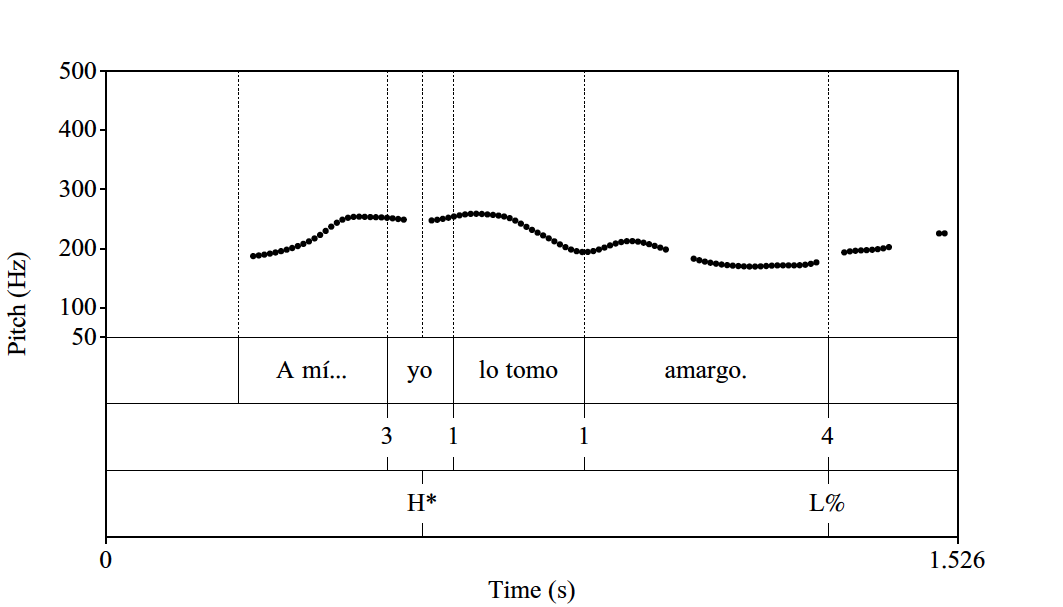
\includegraphics[width=\textwidth]{figures/pes-img17.png}
\caption{F0 contour of the utterance \textit{\textbf{Yo} lo tomo amargo} (‘I drink it bitter’) with a preverbal PS as a contrastive topic, realized with a H*.\label{fig:pes:17}}
 \end{figure} 

 
 \begin{figure}
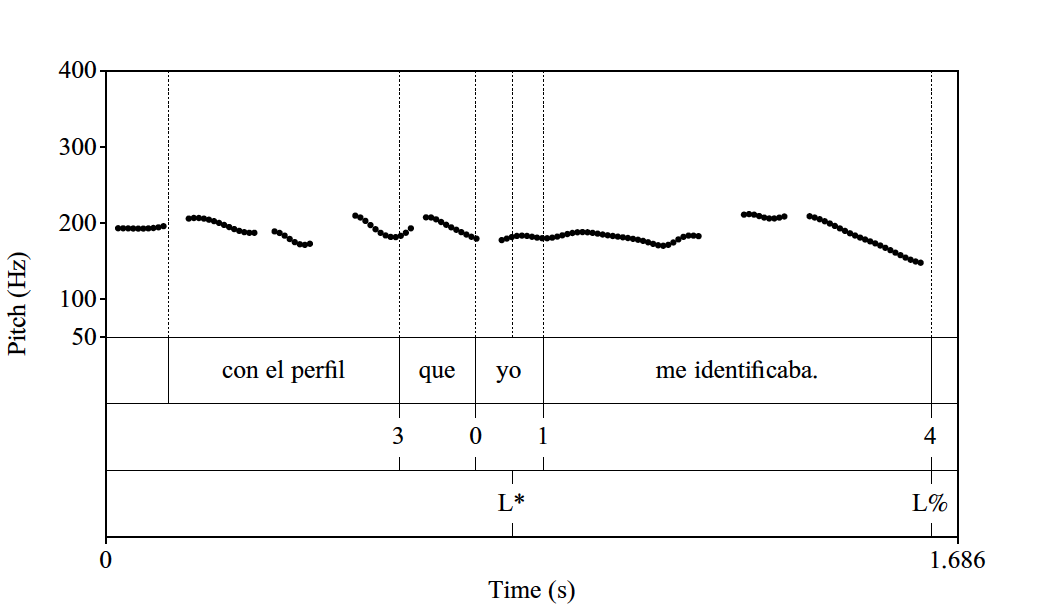
\includegraphics[width=\textwidth]{figures/pes-img18.png}
\caption{F0 contour of the utterance \textit{con el perfil que \textbf{yo} me identificaba} (‘with the profile that I identified with’) with a preverbal PS as a disambiguating topic, realized with an L*.\label{fig:pes:18}}
\end{figure}

Further results indicated that right-dislocated (familiar) topics were always realized as a \isi{low tone} (L*) and separated by a \isi{low boundary tone} (L\textminus{}) from the preceding \isi{prosodic unit} (\figref{fig:pes:19}). 



\begin{figure}
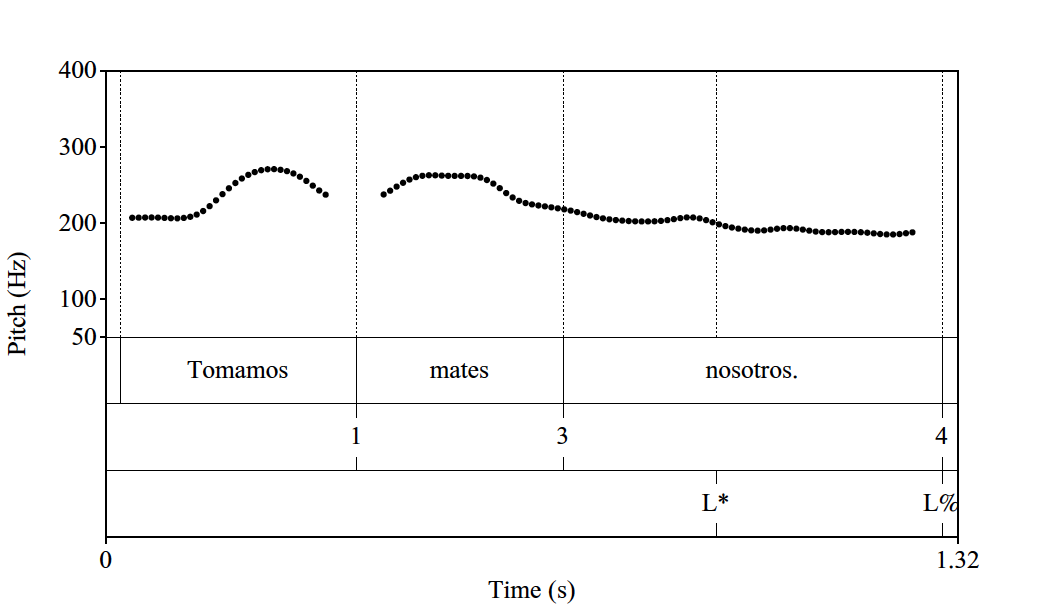
\includegraphics[width=\textwidth]{figures/pes-img19.png}
\caption{F0 contour of the utterance \textit{Tomamos mates \textbf{nosotros}} (‘We drink \textit{mates}’; lit. ‘Drink \textit{mates} we’) with a postverbal PS as a (familiar) topic, realized with an L*.\label{fig:pes:19}}
\end{figure}

It should be noted that a \isi{boundary tone} can be crucial for distinguishing focal PS from subject-topics, which are both realized as an L* in the rightmost position. This shows a complex relationship between the tonal events of a whole sentence. While the focus-domain is separated by a \isi{high tone} (H\textminus{}), the topic-domain is separated by a \isi{low tone} (L\textminus{}) from the preceding \isi{prosodic} material.

And finally, there was another interesting tendency with regard to the peak position of PS when it was compared with pitch accents associated with other words within one \isi{prosodic unit}. Pitch in the less accessible IS categories (F, Tc, Ta) reached the maximal point in one \isi{prosodic} phrase more frequently than in the more accessible IS categories (Tf, Td). For instance, while the focal PS exhibited the highest pitch in 93\% of cases, \is{topic!contrastive}contrastive topic PS in 68\%, and \is{topic!aboutness-shift}aboutness-shift topic PS in 43\%, the pitch of PS as a familiar topic did so in only 33\% of cases, and disambiguating topic in 37\% (\figref{fig:pes:20}). The fact that disambiguating topic was prosodically less ``prominent'' than focal subjects or \is{topic!contrastive}contrastive topics supports the assumption that it represents a kind of familiar or \is{topic!aboutness-shift}aboutness-shift topic whose function is simply to undo referential ambiguities in (semantically unpredictable) contexts.\largerpage[-3]

  
\begin{figure}
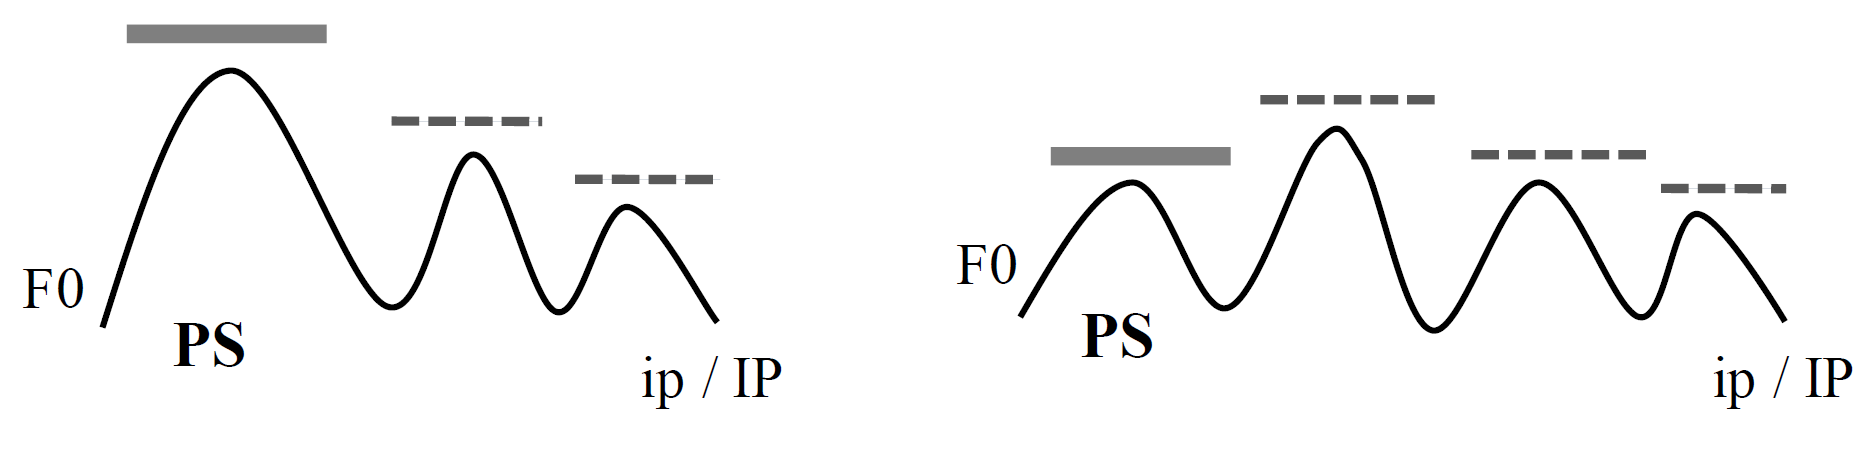
\includegraphics[width=.8\textwidth]{figures/pes-img20new.png}
 \caption{Schematic representation of a prosodic ip/IP unit with a preverbal PS with maximal pitch (left) and non-maximal pitch (right).}
 \label{fig:pes:20}
\end{figure}
 
At this juncture, it is worth mentioning the study by \citet{Rello2012}, who measured different acoustic correlates of pronominal anaphora in ambiguous contexts in \ili{Spanish}. They proposed that a prosodically prominent element should be more accessible for anaphoric reference than a non-prominent one. They found some important differences regarding the duration of pause (which is longer with more distant antecedents than with closer antecedents), as well as the duration of anaphoric pronouns (which are shorter with more distant antecedents). Additionally, the mean F0 range of the anaphoric pronoun is greater when there is a more distant (less accessible) than a closer (more accessible) antecedent. This patterns with the tendencies observed in the present study as well. Hence, further research is needed that examines not only F0 contours but also other \isi{prosodic} parameters such as duration, scaling, tonal level and span, and so on. But even with more in-depth \isi{phonetic} analysis, the question would remain as to what the underlying phonological category is. How can tonal variation be explained and integrated into theories of the grammar of \isi{intonation}? 

As we observed, the present data, not surprisingly, exhibited abundant tonal (inter-speaker as well as intra-speaker) variation, especially in the preverbal non-focal position. I suggest that all the attested tonal realizations of the (preverbal) topics are \isi{phonetic} realizations of the underlying tone /L+H*/, which represents a typical \isi{prenuclear} and/or sentence-initial \isi{accent} in this variety. The tonal variation can have various explanations: the \isi{pitch accent} [L+<H*] was observed mostly in contexts where the subject was followed by a clitic pronoun; in the case of [H*], the leading tone was often unexpressed in contexts of tonal clashes or with \isi{voiceless} consonants; and, finally, the [H+L*] was found systematically after a \isi{high boundary} (H\textminus{}) (seen in \figref{fig:pes:16}). This example shows how \isi{phonetic} realizations can undergo certain phonological processes such as assimilation, by which the \isi{pitch accent} acquires certain features from another tonal event: here we see that as the metrically strong \isi{syllable} occurs directly after a H\textminus{}, the \isi{pitch accent} associated with this \isi{syllable} has a falling pattern affected by the preceding high F0. An abstract (tonal) analysis, taking into account the observed variation in linguistic data, is summarized in \REF{ex:pes:10}\footnote{Additionally, focal PS realized as L+H*, L*, or H* were found in cleft constructions or with focusing adverbs.} and \REF{ex:pes:11}\footnote{The topics in postverbal position were predominantly realized with L* in \isi{declarative} sentences.} (V = Verb).\largerpage

\ea\label{ex:pes:10}
{PS as a focus}\\
\resizebox{\linewidth}{!}{\begin{tabular}{@{}lll@{}}
\multirow{3}{*}{/L+H*+L/  →}  & [L+H*+L]                   &/  {\longrule} L\textminus{} V  (postfocal deaccentuation)\\{}
				&  [L+H*+L], [H+L*], [L*]    &/ V{\longrule} L\%\\{}
				& [L+H*], [L+¡H*]            &/ V{\longrule} H\textminus{} or HL\%\\{}
\end{tabular}}
\z



\ea\label{ex:pes:11}
{PS as a topic}\\
\begin{tabular}{lll}
\multirow{3}{*}{/L+H*/  →}  & [L+H*], [L+<H*], [H*], [L*]                   &/  {\longrule} V \\{}
				&  [H+L*], [H*]    &/ H\textminus{}{\longrule} V\\{}
             
\end{tabular}
\z




%\ea\label{ex:pes:11}
%{PS as a topic}\\
%
%         [L+H*], [L+<H*], [H*], [L*]     /  \_\_ V\\
%     /L+H*/     →  [H+L*], [H*]           /  H- \_\_ V\\
%     \z
     
Let us add that the different pitch accents may represent contrastive units in other contexts, but such contrasts can be neutralized, as can be commonly observed in segmental phonology (e.g. the difference between /r/ and /ɾ/ is neutralized in \ili{Spanish} at the beginning of the word, where only [r] is possible). According to  \citet[13]{Hualde2016}, the occurrence of neutralization is ``even greater in the intonational component. The proper understanding of neutralization phenomena is helped by the recognition of two levels of analysis in addition to surface phonetics.''

At the end of this section, we will come back to the utterance \textit{Yo tomo mucho mate} (\figref{fig:pes:5}), a case where the speaker has insufficient \isi{phonetic} material to implement two pitch accents. We saw that such tonal clashes make an analysis and generalization quite difficult. One methodological possibility for proving the association between a tonal category and a given IS-category would be
(1) to change the material (e.g. use the three-\isi{syllable} \isi{paroxytonic} noun \textit{Rodrigo} instead of the monosyllabic pronoun \textit{yo}),
(2) to place the new material in the exactly same context, and
(3) to let the same speaker produce the sentence. After effecting these changes, the contour in \figref{fig:pes:21} is obtained.

  

\begin{figure}
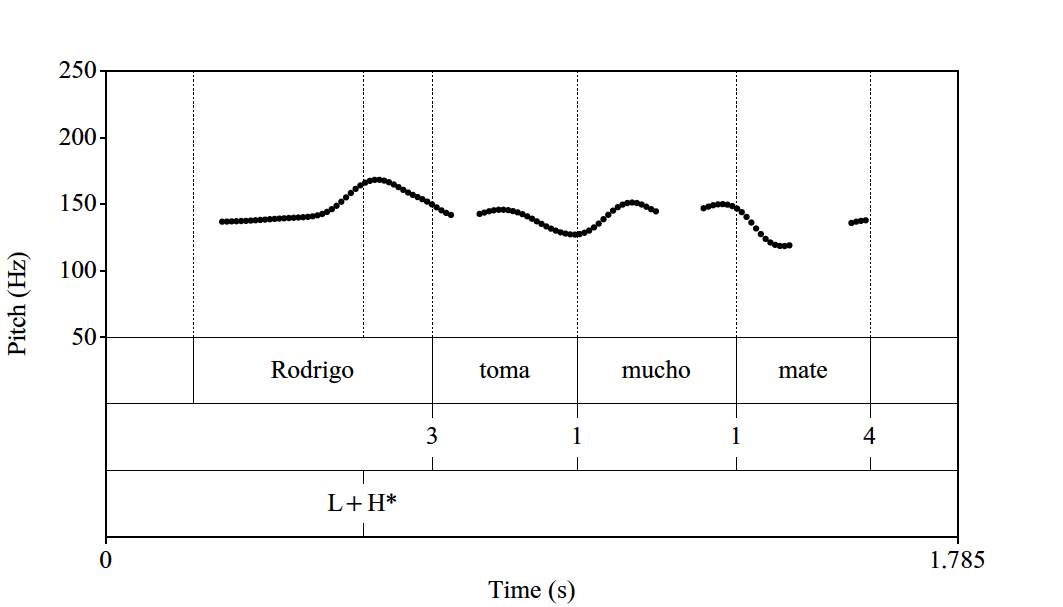
\includegraphics[width=\textwidth]{figures/pes-img21.png}
  \caption{F0 contour of the utterance \textit{Rodrigo toma mucho mate} (‘Rodrigo drinks a lot {mate’}), with an L+H* rising pitch accent.}
  \label{fig:pes:21}
\end{figure}

In this fashion, we could obtain evidence that the same speaker realizes the topic with a rising F0 movement during the $\sigma $* with the F0 peak located at its end (thus, L+H*). Nevertheless, this procedure would involve some sort of artificially prompted elicitation, with all that that implies for the authenticity of the intonational output. Another possibility would be to test by means of different perception experiments whether the two tonal events (set in appropriate contexts) represent contrast or not (see, e.g., \citealt{Vanrell2006,Feldhausen2011,BorrasComes.2014}). Hence, further empirical work is still needed, which ideally would combine a corpus-based (i.e. quantity-based) approach with different experimental laboratory techniques to achieve a better understanding of the tonal categories in natural discourse.


\section{Conclusion}
\label{sec:pes:5}
The objective of the present paper was
(1) to show how intonational analysis can enhance the study of PS with different IS functions in \textit{Porte{\~n}o} \ili{Spanish} (a typically \isi{null-subject language}), and
(2) to discuss the applicability of the ToBI labeling system to the \isi{intonation} of speech obtained from face-to-face free conversations, a traditional sociolinguistic method for studying spontaneous and informal speech.

The study proved by means of intonational analysis that overt PS are not perforce ``emphatic'' or ``contrastive'' categories, as is usually assumed in theoretical studies. Moreover, it was demonstrated that \isi{intonation} together with syntax (here: word order) is relevant in distinguishing topics from focus (L+H* vs. L+H*+L), while contextual conditions play an important role in determining different types of topics. Both of the intonational patterns (L+H*, L+H*+L) found in spontaneous data fit the patterns that have been encountered in semi-spontaneous data on Argentinean \ili{Spanish} in previous research. Besides the typical \is{tritonal pitch accent}tritonal realization, focus can also have other tonal realizations in cases where it is expressed in cleft constructions or with a focal adverb. As for different kinds of topics, the results showed that the prevailing \isi{pitch accent} is a rising L+H*, which may have various \isi{phonetic} realizations, and that there seem to be no strictly consistent (in phonological terms) correlates for such topics in \textit{Porte{\~n}o} \ili{Spanish}.

A second question explored in this paper was the suitability of the (\ili{Spanish}) ToBI labeling system for describing the intonational properties of PS. We have seen and outlined some problems and limitations of the system, regarding especially the treatment of the phonetics-phonology interface in spontaneous data (see, e.g., \citealt{Breen2012}). Nonetheless, in spite of the difficulties presented (e.g. tonal clashes, \isi{voiceless} segments, disfluencies, articulation rate etc.), ToBI can be considered an appropriate and useful tool for \isi{intonation} modeling in \isi{spontaneous speech}, as it allows the user to systematize tonal characteristics and detect patterns of categories in the data. The apparent limitation of the system may serve only as an opportunity for further innovative reanalysis and perhaps a refining of the labels with greater \isi{phonetic} detail.\pagebreak

The observed (inter- as well as intra-speaker) variation, not only in the intonational properties of PS seen here but in the use of PS in general, has sometimes been regarded as either problematic or of little concern for some linguistic theories. But it is important to remember that we can still determine certain patterns across speakers despite such variation. This supports the idea ``that structured linguistic variation is an intrinsic part of speakers’ grammatical knowledge'' (\citealt[xiii]{Carvalho2015}).

Of course, the present study has left many issues unaddressed. Besides leaving out more \isi{phonetic} details, it has not studied emotions, different degrees of expressive force, types of sentences, and other additional factors (such as evidentiality and epistemicity), which might also have an impact on intonational patterns. But I hope that the study has taken—if not an important, at least an interesting—step forward not only in the study of overtly realized PS in \ili{Spanish}, but also in the study of \isi{spontaneous speech} in general.

\section*{Acknowledgments}
I would like to thank Ingo Feldhausen, Jan Fliessbach, and Maria del Mar Vanrell, as well as two anonymous reviewers for their thoughtful observations and very helpful comments. My thanks also go to Uli Reich for his comments on an earlier version of this paper, and Michael Kennedy-Scanlon for checking the English. It goes without saying that all errors remain my own.

{\sloppy
\printbibliography[heading=subbibliography,notkeyword=this]
}

\end{document}
